\chapter[Voronoi Analysis of Quasi\--Two\--Dimensional Hard Spheres]{Voronoi Analysis of \\ Quasi\--Two\--Dimensional \\ Hard Spheres} 
\label{ch:quasi2d}

\begin{chapterabstract}
Experimental investigations have led to the synthesis of colloidal monolayers, where particles are sedimented on a surface, creating effective quasi\--two\--dimensional hard sphere systems.
Voronoi diagrams are constructed for a range of configurations of such systems, generated from both experiment and computation.
The evolution in the network properties with packing fraction is explored for mono, bi and polydisperse particle systems.
A detailed comparison is presented of unweighted and weighted variants of the Voronoi construction in the context of quasi\--two\--dimensional systems.
It is shown that the \td{} unweighted Voronoi, favoured in experimental analyses, has a well\--defined physical interpretation, corresponding to the basal section through a three\--dimensional weighted Voronoi.
In addition the stereology of the three\--dimensional Voronoi is examined and constrasted with equivalent systems of hard disks.
\end{chapterabstract}

\section{Quasi\--2D Hard Sphere Systems}

Hard particle models are a central tenet of statistical physics, forming the basis of fundamental research dating from the earliest computations to current research \cite{Isobe2016}.
This is because, despite their simplicity, the hard disk and hard sphere models are able to explain many of the behaviours of classical particles in two and three dimensions.
In particular, these models effectively complement the study of colloids \cite{Pusey1986}.
The interest in colloids themselves stems from the fact that they occupy a ``sweet\--spot'', in that the particles are large enough to observe with confocal microscopy, whilst being small enough that their motion is governed by simple fundamental forces on a reasonable time scale. 
It is therefore possible to track and visualise particle positions in real\--time, also making them an good proxy for classical atomic systems.

The hard particle model was introduced in section  \ref{s:hardparticlemodelintro}, in the context of hard disks and hard spheres, which, as mentioned, have been extensively studied in the literature.
However, section \ref{s:genexpnetworks} introduced a new system of recent experimental interest, that of a monolayer of hard spheres.
These systems, where colloidal particles are sedimented on a plane in a single layer, are \thd{} (3D) systems with effectively \td{} (2D) interactions.
As such, they are termed quasi\--\td{} (\qtd{}).
In section\ref{s:hardparticlemodelintro}, all monolayers comprised spheres of the same size, but one can equally engineer systems where the sphere radii have a distribution of sizes \ie{} different size dispersity \cite{Thorneywork2014,Thorneywork2018}.
In the polydisperse case, the centres of the spheres no longer lie in the same plane, but rather at a height equal to their radius.
The result of this dispersity is that the interaction distances between particles of different sizes cannot be trivially projected into 2D.
Nevertheless, it is still possible to model monolayers of spheres in 2D by using non\--additive distances.
For two particles in a \qtd{} arrangement with radii, $R_i$, the contact distance in 2D, $R_{ij}$, is related to the geometric mean of the radii:
\begin{equation}
	R_{ij}=2\left(R_iR_j\right)^{1/2}\,,
\end{equation}
as  illustrated for two spheres, $A$, $B$, in figure \ref{fig:nonadddemo}.
Alternatively, this can be expressed in terms the arithmetic mean and a non\--additivity parameter, $\Delta$, as is common for asymmetric systems \cite{Roth2001}:
\begin{equation}
	R_{ij}=\left(R_i+R_j\right)\left(1+\Delta\right)\,,
\end{equation}
where
\begin{equation}
	\Delta=\frac{2\left(R_iR_j\right)^{1/2}}{R_i+R_j}-1\,.
\end{equation}
This allows \qtd{} systems to be modelled purely in 2D.

\begin{figure}[bth]
     \centering
     
     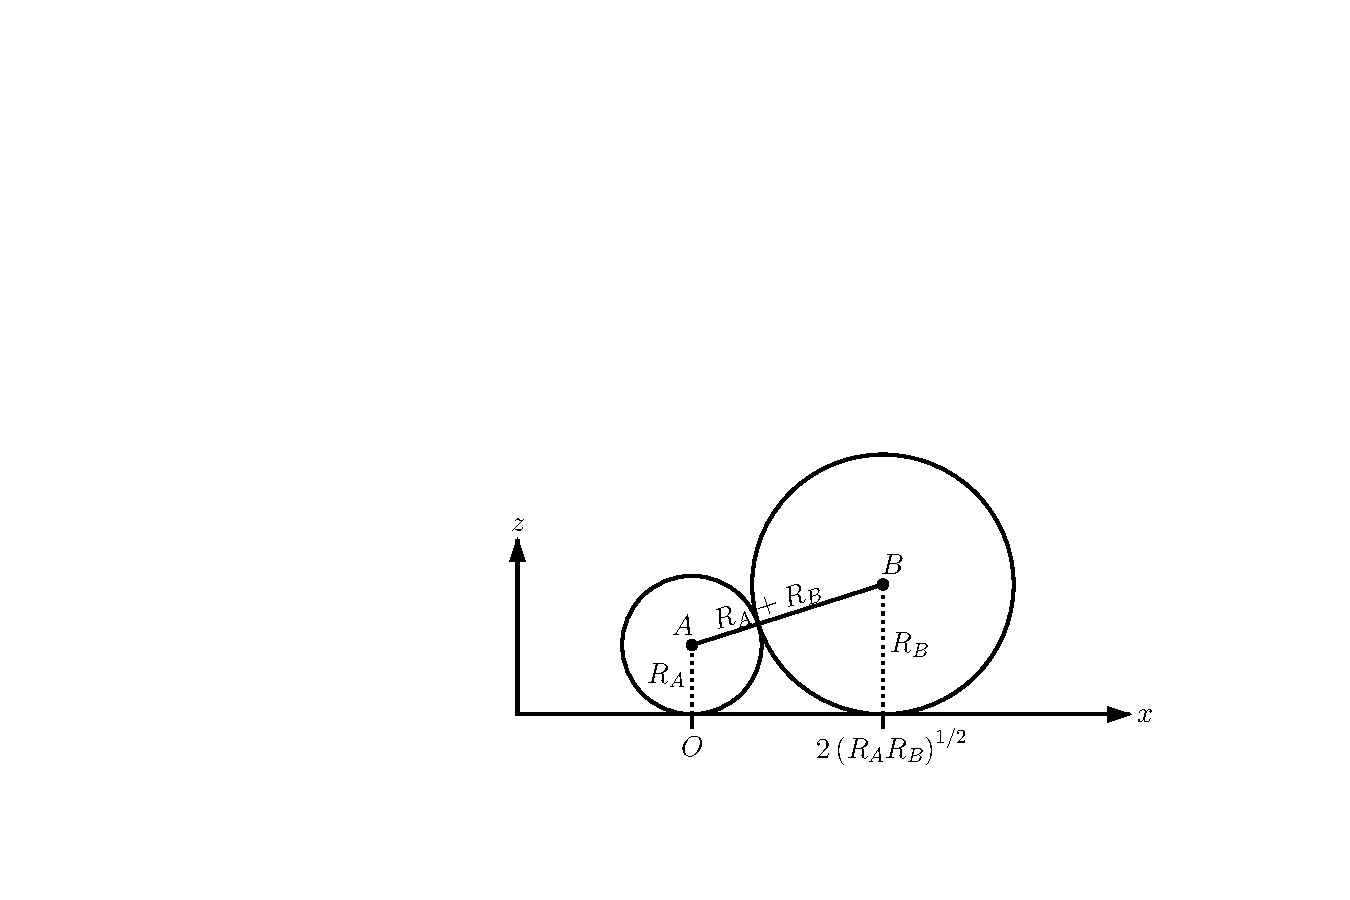
\includegraphics[width=10cm]{./figures/quasi2d/quasi2d_a.pdf}
     \caption{Quasi\--2D hard spheres can be modelled in 2D by using non\--additive interaction distances. Here two spheres sedimented on a plane have a contact distance given by twice the geometric mean of the radii.}
     \label{fig:nonadddemo}
\end{figure}

Since systems of colloidal monolayers can be treated as a 2D problem, this should enable them to be analysed with a 2D Voronoi diagram.
Voronoi analysis allows determination of the coordination environments around each particle, so that network properties such as the neighbour degree distribution and correlations can be calculated \cite{Earnshaw1994,Yang2002,Kumar2005,Chremos2007}.
This information can be used, for example, to give insights as to the phase behaviour in these systems \cite{Jaster1999,Pronk2004,Kapfer2015,Thorneywork2017}.
However, it is not initially clear how the non\--additivity will affect the calculation of the Voronoi diagram.
For instance, unlike a system of additive hard disks, it is not obvious if a unweighted or weighted variant of the Voronoi construction is most appropriate, and in the latter case what the weightings should be.
It will be demonstrated in the second half of this chapter that in fact the unweighted construction retains a precise physical meaning for \qtd{} systems, and is the natural choice for partitioning space in these monolayers.

\subsection{Experimental Analysis}

Raw experimental coordinates were kindly provided for a range of mono\-- and bidisperse colloidal systems by Thorneywork and Dullens \cite{Thorneywork2014,Thorneywork2017,alice2015a}.
The colloidal monolayers were prepared by dispersing particles of specific radii in a water\--ethanol mixture and sedimenting them on the base of a glass sample cell.
The samples were then imaged using an inverted bright-field microscope and particle coordinates obtained using standard particle tracking routines.
Allowing a time of around $~10s$ between frames ensured that the particle positions are sufficiently decorrelated to be statistically independent. 

\begin{table}
\centering
\caption{Summary of the experimental parameters which can be controlled in colloidal monolayers.}
\label{tab:expcolloidparams}
\begin{tabular}{@{}cccccc@{}}
\toprule
& \multicolumn{1}{c}{Mono} & \phantom{x} & \multicolumn{3}{c}{Binary} \\ 
\cmidrule{2-2} \cmidrule{4-6} 
& & & Large & Small & Total \\ 
\midrule
Radius & $R$ & & $R_l$ & $R_s$ & - \\
Radius ratio & 1 & & - & - & $\gamma=R_l/R_s$ \\
Composition & 1 & & $c_l$ & $c_s$ & 1 \\
Number density & $\rho$ & & $\rho_l=c_l\rho$ & $\rho_s=c_s\rho$ & $\rho=\rho_l+\rho_s$ \\
Packing fraction & $\phi=\rho\pi R^2$ & & $\phi_l=\rho_l\pi R_l^2$ & $\phi_s=\rho_s\pi R_s^2$ & $\phi=\phi_l+\phi_s$ \\
\bottomrule
\end{tabular}
\end{table}

Data was made available across a range of experimental conditions.
For the monodisperse systems, samples contained particles with radii of $R=1.395\mu$m, across a range of 2D packing fractions, $\phi$, as defined in equation \eqref{eq:packingfraction}.
For bidisperse systems, which consist of two particle sizes, one ``large'' and the other ``small'', there are more free parameters to control, which are summarised in table \ref{tab:expcolloidparams}.
Firstly there is the radius ratio of the particles, $\gamma=R_l/R_s$ (the subscripts ``$l$'' and ``$s$'' will be used to denote variables corresponding to large and small particles respectively), which relates the relative particle sizes.
Secondly, the composition, $c_l$, $c_s$, determines the proportion of each particle type, where $c_l+c_s=1$.
Finally there is also the packing fraction, calculated with reference to one of the components $\phi_l$, $\phi_s$, or using all particles to give a total packing fraction $\phi=\phi_l+\phi_s$.
For completeness, it is noted that the composition can also be represented by $\phi_l/\phi$, but for the purposes of this work the definition above was found to be more intuitive.
The available experimental data contained systems at two radius ratios and a variety of compositions and packing fractions.
More specifically, these had either $R_s=1.395\mu$m and $R_l=3.05,2.02\mu$m, corresponding to size ratios of $\gamma=2.19, 1.45$ respectively.
In addition for each set of experimental conditions there were 100 configurations, which the exact compositions and packing fractions for each were determined and presented in table \ref{tab:expcolloid}

\begin{table}
\centering
\caption{Details of experimental colloidal samples. Samples are defined in terms of particle size dispersity, particle radius ratio, composition and total packing fraction. The mean value is supplied for each, with the standard deviation given in brackets.}
\label{tab:expcolloid}
\begin{tabular}{@{}ccccccccccc@{}}
\toprule
\multicolumn{1}{c}{Mono} & \phantom{x} & \multicolumn{2}{c}{Binary, $\gamma=2.19$} & \phantom{x} & \multicolumn{2}{c}{Binary, $\gamma=1.45$} & \phantom{x} & \multicolumn{2}{c}{Binary, $\gamma=1.45$}\\ 
\cmidrule{1-1} \cmidrule{3-4} \cmidrule{6-7} \cmidrule{9-10}
$\phi$ & & $c_l$ & $\phi$ &  & $c_l$ & $\phi$ & & $c_l$ & $\phi$  \\ 
\midrule
$0.655(1)$&&$0.201(1)$&$0.764(2)$&&$0.532(4)$&$0.571(1)$&&$0.233(1)$&$0.607(2)$\\
$0.616(1)$&&$0.182(1)$&$0.639(2)$&&$0.522(4)$&$0.477(4)$&&$0.208(1)$&$0.406(1)$\\
$0.509(1)$&&$0.192(2)$&$0.507(3)$&&$0.543(5)$&$0.267(1)$&&$0.226(3)$&$0.309(2)$\\
$0.427(1)$&&$0.189(2)$&$0.339(3)$&&$0.332(1)$&$0.629(1)$&&$0.091(1)$&$0.663(1)$\\
$0.341(1)$&&$0.187(7)$&$0.150(2)$&&$0.314(3)$&$0.499(3)$&&$0.107(1)$&$0.500(2)$\\
$0.289(0)$&& &&&$0.345(2)$&$0.337(2)$&&$0.087(1)$&$0.257(1)$\\
\bottomrule
\end{tabular}
\end{table}

The 2D experimental coordinates can be analysed using a Voronoi construction. An example for both a mono and bidisperse configurations can be found in figure \ref{fig:expvoro}.
With the raw coordinates, the experimental samples can be treated analogously to configurations generated from computation.
The only difference is that the experimental images are by nature aperiodic, and so when analysing the network properties of the Voronoi diagram, the cells close to the boundary must be neglected, to remove any edge effects. 
However, careful examination of figure \ref{fig:expvoro1} reveals some small imperfections in the data, as there are instances where the monodisperse particles appear to overlap.
This is not a result of differences in particle size, but rather the presence of ``phantom'' particles deriving from the imaging process.
Extracting particle positions from the experimental data is highly non\--trivial, in particular removing points arising from interstitial sites between densely packed particles \cite{alice2015a}.
Whilst this becomes more problematic at higher packing fractions, they are however still few and far between.
It should also be point out here that the tracking routines are able to detect the difference between large and small particles in bidisperse systems, allowing Voronoi cells to be associated to particles of a specific size.
The actual results of the analysis of these experimental systems will be discussed alongside the results from computation in section \ref{s:monodisperse} and \ref{s:bidisperse}.

\begin{figure}[bt]
     \centering
     
      \begin{subfigure}[b]{0.48\textwidth}
         \centering
         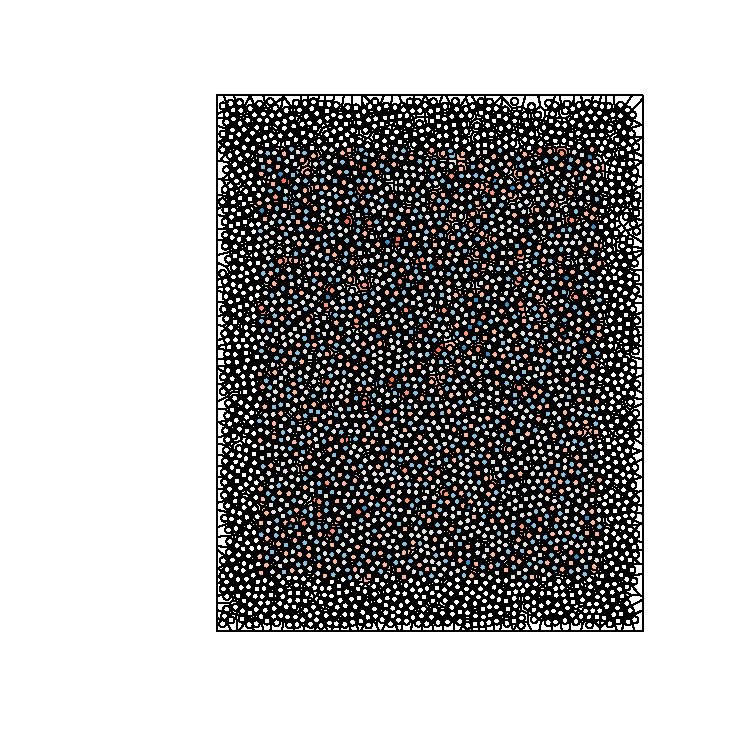
\includegraphics[width=\textwidth]{./figures/quasi2d/exp_mono.pdf}
         \caption{Mono, $\phi=0.509$}
         \label{fig:expvoro1}
     \end{subfigure}
     \hfill
       \begin{subfigure}[b]{0.48\textwidth}
         \centering
         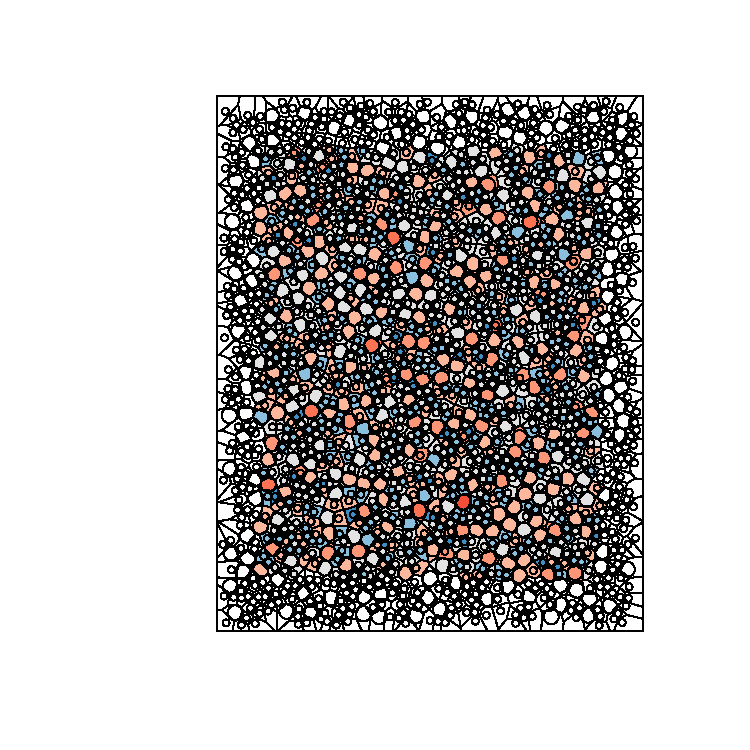
\includegraphics[width=\textwidth]{./figures/quasi2d/exp_lsr.pdf}
         \caption{Binary, $\gamma=2.19$, $c_l=0.192$, $\phi=0.507$}
         \label{fig:expvoro2}
     \end{subfigure}
     \hfill
     
     \caption{Voronoi analysis of two example experimental snapshots, of a monodisperse and bidisperse \qtd{} colloidal monolayer (system parameters in captions). Circles indicate particles of a given radius whilst Voronoi cells are coloured according to size. Voronoi cells without shading indicates those that were neglected from network analysis due to proximity to the image boundary.}
     \label{fig:expvoro}
\end{figure}

\subsection{Non\--Additive Hard Disk Monte Carlo}
\label{s:nonaddmc}

Experimental data can be compared and contrasted with configurations generated from simulation.
Hard particle \mc{} was introduced in section \ref{s:hardparticlemc} as a method to generate such configurations computationally.
One could set up a 3D system of hard spheres constrained to a plane, but as discussed above it is preferable to employ a non\--additive hard disk model.
In this modification, if two particles are separated by a distance, $r_ij$, the pair potential is:
\begin{equation}
	\mathcal{U}_{ij} = \begin{cases} \infty \quad &r_{ij}<2\left(R_iR_j\right)^{1/2} \\ 0 \quad &\text{otherwise} \end{cases}\,.
\end{equation}
The remainder of the algorithm proceeds the same as in the standard methods, as outlined in section \ref{s:hardparticlemc}.

For all simulations in this chapter, unless otherwise stated, $\mathcal{N}=1000$ particles were placed in a 2D periodic box, then equilibrated with $10^5$ Monte Carlo cycles with each cycle consisting of $\mathcal{N}$ random moves.
After equilibration, $10^5$ Monte Carlo cycles are performed with sampling every $100$ cycles.
For each set of simulation parameters, averaging was carried out over 10 different random seeds.


\section{Monodisperse Spheres}
\label{s:monodisperse}

The simplest \qtd{} system to study is that of a monolayer of monodisperse spheres.
This is because as all sphere radii are the same, the non\--additive model reduces here to a simple additive model of hard disks.
The case of monodisperse spheres has therefore already been partially explored the previous chapter.
For example, sections \ref{s:gendegreedist} and \ref{s:genassortativity} discussed the degree\--distributions and assortativity in contrast with a range of other physical networks.
To avoid repetition, this section will therefore focus on the network properties in terms of a measure specific to colloids, the packing fraction.

\subsection{Network Properties with Packing Fraction}

The network properties of the Voronoi diagrams in this section are again summarised by the proportion of hexagons, $p_6$, and the assortativity, $r$.
As was shown in section \ref{s:gendegreedist}, as the ring statistics in the Voronoi diagrams of monodisperse \qtd{} colloids follow \lm's maximum entropy law, $p_6$ can also be considered a descriptor for the width of the ring distribution.
The assortativity once again measures the local ring correlations.
Figure \ref{fig:mono1} shows the results of the evolution of $p_6$ with $\phi$, for both experiment and simulation.
The first thing to note is that there is excellent agreement between the experimental system and the hard particle model, indicating that this model is indeed suitable for exploring the behaviour of colloidal monolayers.
In addition, comparison is also provided to a previous computational study \cite{Kumar2005}, to which again there is perfect agreement.
More generally, the value of $p_6$ decreases with packing fraction.
The hexatic phase, which exists at high packing fraction is characterised by having particles in 6\--coordinate environments.
Under melting, as the available volume increases, 5\-- and 7\--ring defects are initially introduced, depreciating $p_6$, before more extreme ring sizes manifest.
Finally, in the limit of the ideal gas (as $\phi\rightarrow 0$), the Poisson Voronoi tessellation is obtained.

The behaviour of the assortativity with packing fraction is given in figure \ref{fig:mono2}.
Once again, there is very good agreement between configurations from experiment and computation.
The fluctuations in the values of $r$ are larger than $p_6$, for the experimental systems.
\davidnote{Todo: rationalise these fluctuations}.
Strikingly, the assortativity seems to display behaviour that is linear in packing fraction, at least for intermediate values.
It is not immediately clear why this should be the case, and is an interesting result that warrants more research.
In addition, it can be seen that this linearity comes to an end around $\phi\approx 0.66$, with $r$ displaying a sudden upturn.
This point is close to the limit of the liquid phase for hard disks, before it undergoes transition to a hexatic phase \cite{Thorneywork2017}.
This phase transition seems to be captured clearly through the assortativity.

\begin{figure}[bt]
     \centering
     
      \begin{subfigure}[b]{0.45\textwidth}
         \centering
         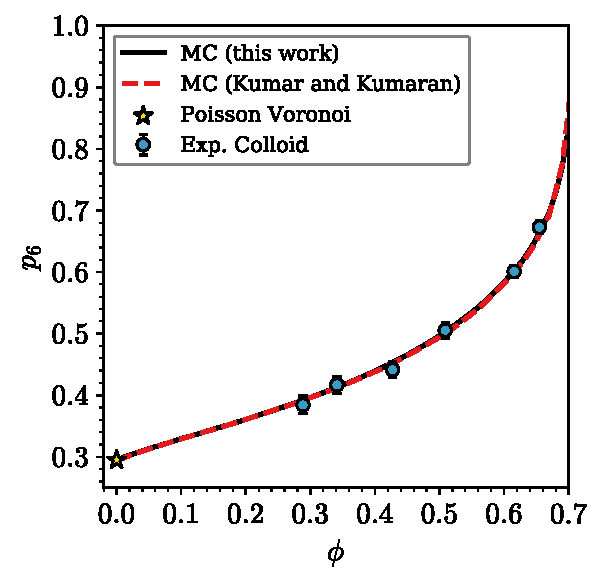
\includegraphics[width=\textwidth]{./figures/quasi2d/mono_phi_p6.pdf}
         \caption{}
         \label{fig:mono1}
     \end{subfigure}
     \hfill
       \begin{subfigure}[b]{0.48\textwidth}
         \centering
         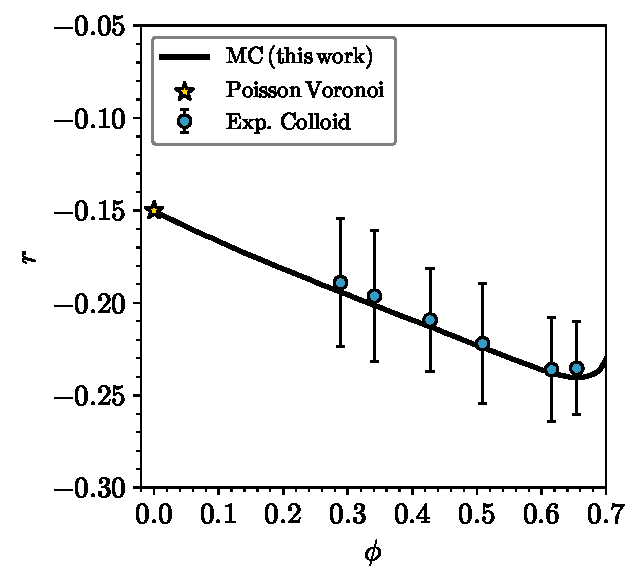
\includegraphics[width=\textwidth]{./figures/quasi2d/mono_phi_r.pdf}
         \caption{}
         \label{fig:mono2}
     \end{subfigure}
     \hfill
    
     \caption{Network properties of monodisperse systems of \qtd{} hard spheres, in terms of the proportion of hexagons, panel (a), and the assortativity, panel (b). Data is presented both from simulation and experiment, with the experimental points indicating the mean value and one standard deviation. A comparison is also made in panel (a) to a previous study \cite{Kumar2005}, to which there is excellent agreement.}
     \label{fig:mono}
\end{figure}


\section{Bidisperse Spheres}
\label{s:bidisperse}

Monolayers of bidisperse spheres present a natural extension to the monodisperse case, and come with the advantage of having available experiment information for comparison.
In this section the ring statistics of bidisperse systems will be explored, with a focus on systems matching the experimental parameters, as outlined in table \ref{tab:expcolloid}.
Owing to the fact that there are two types of particle present (which experimental imaging is able to differentiate), metrics in this section will be considered in reference to both large and small particles.
To this point, the ring statistics can then be divided into partial ring distributions for each particle type, denoted $p_k^l$ and $p_k^s$.
A subtle but important point is that the mean ring sizes for these partial distributions ($\ki_l$ and $\ki_s$) are no longer constrained to be six.
Instead it is their weighted sum which is constrained by Euler's formula such that:
\begin{equation}
	c_l\ki_l+c_s\ki_s = \ki = 6\,.
\end{equation}
The mean ring sizes can then take values either side of six, quantifying the relative coordination numbers of the particles of different sizes.

In this section systems of two radius ratios will be discussed: the first with $\gamma=1.45$, termed the small size ratio; the second with $\gamma=2.09$, termed the large size ratio.
The primary focus will however be on the small size ratio, as this is complemented by the most experimental data.
The overarching properties of the ring structure will first be explored, before the explicit ring statistics are again examined in relation to a maximum entropy solution.


\subsection{Ring Statistics with Packing Fraction}

\begin{figure}[bt]
     \centering
     
      \begin{subfigure}[b]{0.48\textwidth}
         \centering
         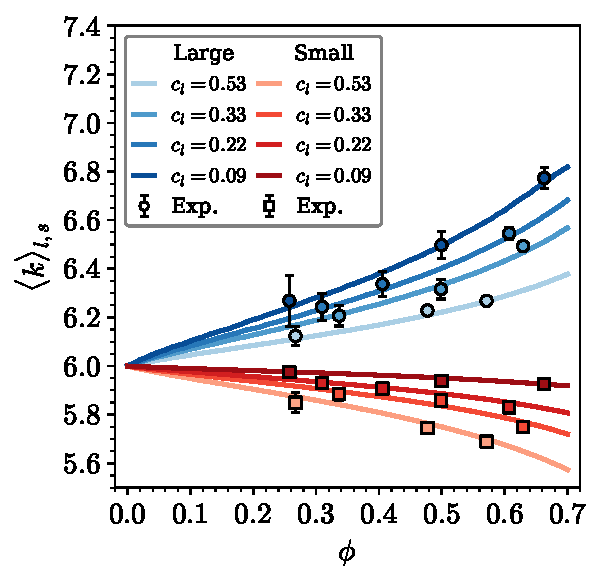
\includegraphics[width=\textwidth]{./figures/quasi2d/bi_ssr_phi_k.pdf}
         \caption{$\gamma=1.45$}
         \label{fig:bi1}
     \end{subfigure}
     \hfill
      \begin{subfigure}[b]{0.48\textwidth}
         \centering
         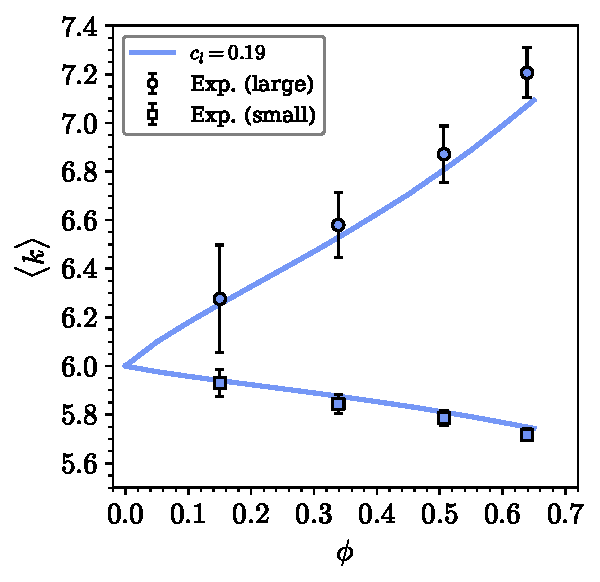
\includegraphics[width=\textwidth]{./figures/quasi2d/bi_lsr_phi_k.pdf}
         \caption{$\gamma=2.19$}
         \label{fig:bi2}
     \end{subfigure}
     \hfill
     
      \begin{subfigure}[b]{0.48\textwidth}
         \centering
         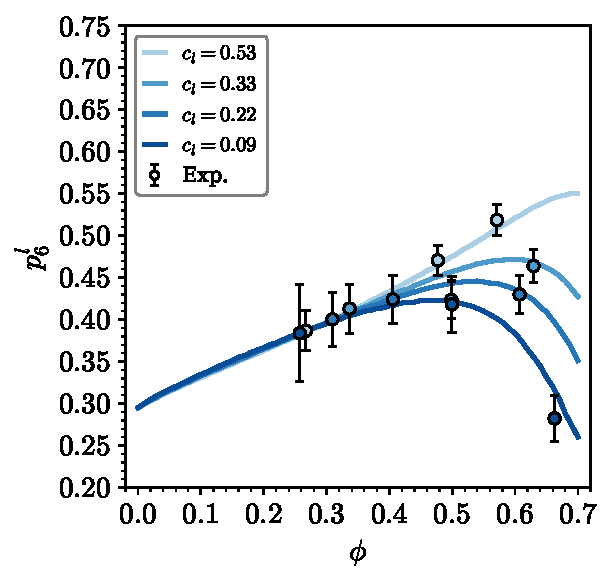
\includegraphics[width=\textwidth]{./figures/quasi2d/bi_ssr_l_phi_p6.pdf}
         \caption{$\gamma=1.45$, large spheres}
         \label{fig:bi3}
     \end{subfigure}
     \hfill
     \begin{subfigure}[b]{0.48\textwidth}
         \centering
         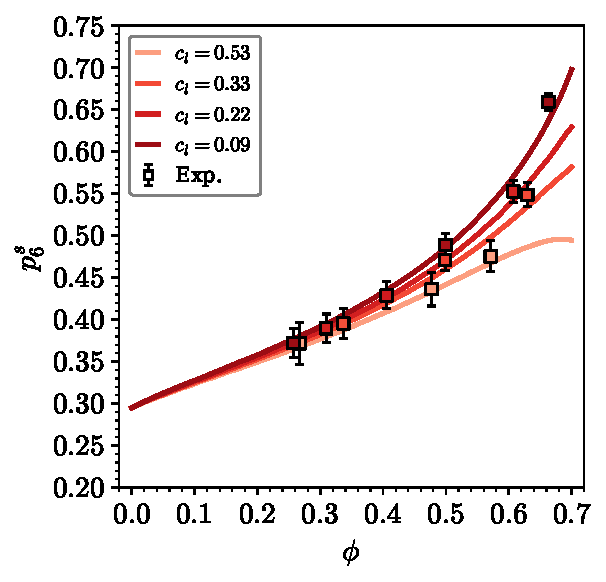
\includegraphics[width=\textwidth]{./figures/quasi2d/bi_ssr_s_phi_p6.pdf}
         \caption{$\gamma=1.45$, small spheres}
         \label{fig:bi4}
     \end{subfigure}
     \hfill
    
     \caption{Overview of the evolution in the partial ring statistics in bidisperse colloidal monolayers. Panels (a),(b) show the partial mean sizes for the two radius ratios (as indicated in captions). Panels (c),(d) show the proportion of hexagons in the partial distributions for the $\gamma=1.45$ systems. The blue curves correspond to quantities pertaining to large particles, red curves to small particles. The system composition is indicated by the depth of shading, as in the legends. Experimental points are coloured using the same scale as for simulation curves, and error bars indicate one standard deviation of the mean.}
     \label{fig:bi}
\end{figure}

The mean values of the partial ring distributions for large and small spheres are given for the bidisperse systems of both radius ratios in figures \ref{fig:bi1}, \ref{fig:bi2}.
Beginning with the small size ratio ($\gamma=1.45$, figure \ref{fig:bi1}), it can be seen that there is once again good agreement with the experimental data.
With the aid of the \mc{} simulations, it is clear that these experimental points actually lie on a series of curves.
To rationalise the broad behaviour of these curves, one can begin by noting that $\ki_l>6$ and $\ki_s<6$ for all values of $\phi>0$.
This is simply an expression of the fact that larger spheres will always have on average more nearest neighbours than smaller spheres.
Following this observation, it can be seen that $\ki_l$ increases as the fraction of large particles decreases, for a fixed packing fraction.
This is a due to large spheres having statistically fewer large sphere neighbours the lower the concentration $c_l$.
Each large particle can accommodate more particles around it, the greater the dilution of small particles.
As a further illustration, one can consider a large sphere in a ``sea'' of small spheres ($c_l\rightarrow 0$).
Here the large particle nearest neighbours must be maximised and equally the small particles only interact with other small particles.
As such the mean coordination for the small particles must approach the average of six.
This reciprocal behaviour of small spheres also explains the trend in $\ki_s$, which approaches the horizontal limit of $\ki_s=6$ as $c_l\rightarrow 0$.
Once again the effect of decreasing packing fraction is to diminish the effects of relative sphere size, as the excluded volume is lower, until eventually the random limit is reached.

The analogous data is also presented for the large size ratio system in figure \ref{fig:bi2}.
Here it can be seen that similar trends hold for $\ki_l$ and $\ki_s$ as discussed for the small size ratio above. 
However, the increased size differential leads to even more extreme differences in the partial mean ring sizes.
For example, for the large size ratio with $c_l=0.19$, $\ki_l\approx7.21$ but for the small size ratio with $c_l=0.22$, $\ki_l\approx6.68$.
It should be noted that the fit with experiment is less accurate for the large size ratio spheres, a problem that is particularly pronounced at higher packing fractions.
This suggests two possible inadequacies.
Either the hard particle model is insufficient, and there are some additional short range interactions which become non\--negligible at higher packing fractions, or the difficulties in directly imaging the particles become more significant. 

The proportion of hexagons for each subsystem is also plotted in terms of the packing fraction in figures \ref{fig:bi3}, \ref{fig:bi4}, for the spheres with small size ratio.
Again, even at this more fine\--grained level, the correlation with experimental data remains strong.
The results for the small spheres in figure \ref{fig:bi4} reflect a general trend regularly seen in this thesis, where the number of hexagons is maximised as ordering increases with higher packing fraction, and again the $p_6$ increases as the number of disrupting large spheres decreases.
The results for the large spheres in figure \ref{fig:bi3} are somewhat more dramatic, with $p_6$ displaying a maximum with changing packing.
This will be discussed to greater extent in the following section, but essentially results from the hexagon no longer being the dominant ring size, begin replaced by the heptagon.
Similar trends were in fact seen for 5\-- and 7\--rings in $\br{4}{10}$ triangle rafts in section \ref{s:triraftnetprop} and figure \ref{fig:trpk3}. 

\subsection{Maximum Entropy Solutions}

\begin{figure}[bt]
     \centering
     
      \begin{subfigure}[b]{0.48\textwidth}
         \centering
         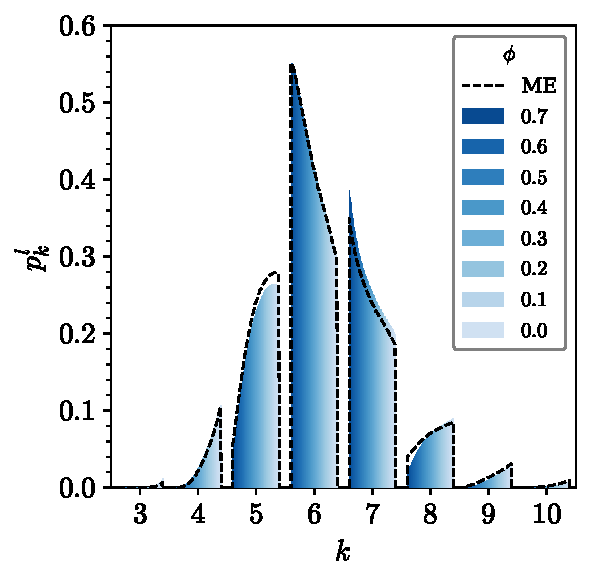
\includegraphics[width=\textwidth]{./figures/quasi2d/phi_me_l_53.pdf}
         \caption{$\gamma=1.45$, $c_l=0.53$, \\large spheres}
         \label{fig:bime1}
     \end{subfigure}
     \hfill
      \begin{subfigure}[b]{0.48\textwidth}
         \centering
         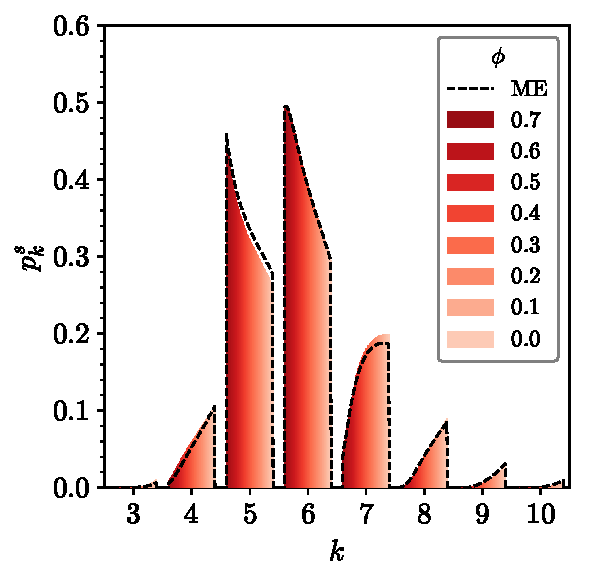
\includegraphics[width=\textwidth]{./figures/quasi2d/phi_me_s_53.pdf}
         \caption{$\gamma=1.45$, $c_l=0.53$, \\small spheres}
         \label{fig:bime2}
     \end{subfigure}
     \hfill
     
      \begin{subfigure}[b]{0.48\textwidth}
         \centering
         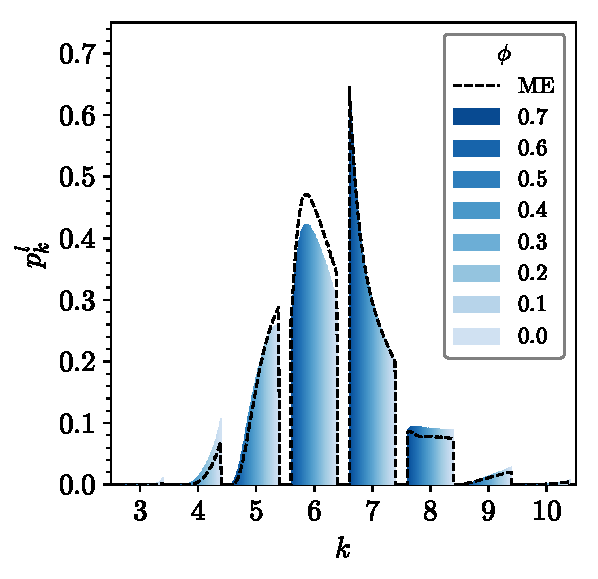
\includegraphics[width=\textwidth]{./figures/quasi2d/phi_me_l_9.pdf}
         \caption{$\gamma=1.45$, $c_l=0.09$, \\large spheres}
         \label{fig:bime3}
     \end{subfigure}
     \hfill
     \begin{subfigure}[b]{0.48\textwidth}
         \centering
         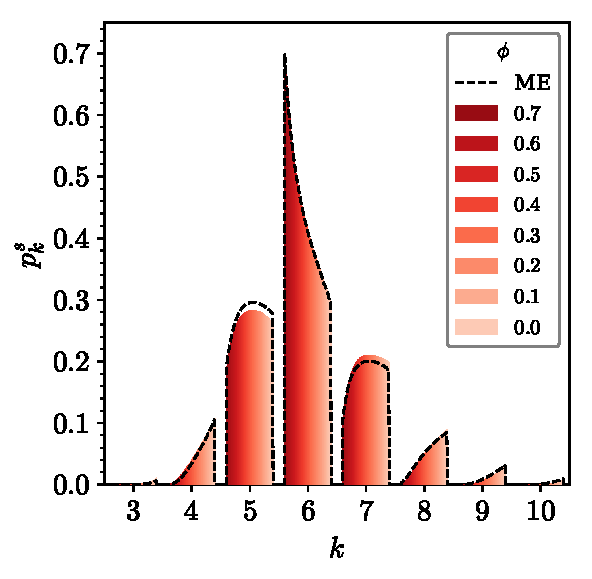
\includegraphics[width=\textwidth]{./figures/quasi2d/phi_me_s_9.pdf}
         \caption{$\gamma=1.45$, $c_l=0.09$, \\small spheres}
         \label{fig:bime4}
     \end{subfigure}
     \hfill
    
     \caption{Variation of partial ring distributions with packing fraction for two different compositions of a $\gamma=1.45$ bidisperse monolayer, contrasted with maximum entropy solutions. Left panels show the statistics for rings associated with larger particles, and right panels with smaller particles. The maximum entropy solutions are overlaid as dashed lines for comparison.}
     \label{fig:bime}
\end{figure}

To further investigate the ring statistics in bidisperse colloidal monolayers, the numerical partial ring size distributions are compared to maximum entropy solutions.
These maximum entropy solutions to are assumed to follow the same form as \lm's law, \ie{} satisfy the constraints:
\begin{align}
	\sum_k p_k &= 1\,, \\
	\sum_k kp_k &= \langle k \rangle_{l,s}\,, \\
	\sum_k \frac{p_k}{k} &= \text{constant}\,.
\end{align}
Unlike \lm's law, which requires only the value of a single ring, such as $p_6$, to obtain the entire distribution, the additional freedom afforded to the mean ring size means that here the mean ring size of the partial distributions must also be provided.

The comparison of the partial ring statistics from simulation and maximum entropy is given in figure \ref{fig:bime}.
The partial distributions are provided for the large and small spheres, with a small size ratio, at the two limiting compositions of $c_l=0.53,0.09$.
The continuous evolution in the ring statistics with packing fraction is detailed by the shading of the bars (note for instance that the $k=6$ bars in figure \ref{fig:bime} are the reverse of the lines of $p_6^{l,s}$ in figures \ref{fig:bi3}, \ref{fig:bi4}).
In these plots, the left\--most points in each bar represent the system at the highest packing fraction, and the right\--most points the limit of zero packing fraction.
In all cases, the maximum entropy solutions fit the observed numerical results quite well.
The difference in the ring statistics for each component is also stark.
For the $c_l=0.53$ system, which is roughly equal in large and small spheres, although at high packing fraction $p_6$ is comparable in magnitude, the distribution for large spheres is skewed heavily towards large rings (particularly $k=7$), whereas that for the small spheres is skewed towards small rings (particularly $k=5$).
For the $c_l=0.09$ system, the distribution for the large spheres is even more dramatic, being dominated at high packing fraction by $7$\--rings.
This causes the value of $p_6$ to exhibit a maximum in $\phi$, as the proportion initially rises as $7$\--rings decay, before heading towards the PV limit.
One might think that this necessarily must also enforce the small sphere distribution to be more ``extreme'', but in fact the reverse is true.
As the small spheres interact primarily with other small spheres, due to their high relative abundance, the ring distribution actually appears more similar to that of the monodisperse case.
Hence, in this way, the two effects offset each other, so that by extremising the distribution of one component, the other must become more regular.

\section{Voronoi Construction in Quasi\--2D}

The case of \qtd{} polydisperse spheres is a further generalisation of the mono\-- and bidisperse systems discussed already in this chapter.
Owing to this generality, a different approach will be taken here, with the meaning of the Voronoi diagram carefully examined in the context of \qtd{} hard sphere systems, before numerical results are presented for polydisperse spheres.
The motivation for this is that up to this point, it has merely been stated that the unweighted 2D Voronoi is an appropriate construction (as opposed to a weighted variant - see section \ref{s:voronoiintro}), even for collections of particles of varying radii.
The opportunity will now be taken to explore this claim more fully.

\begin{figure}[tb]
	\centering
     
      \begin{subfigure}[b]{0.45\textwidth}
         \centering
         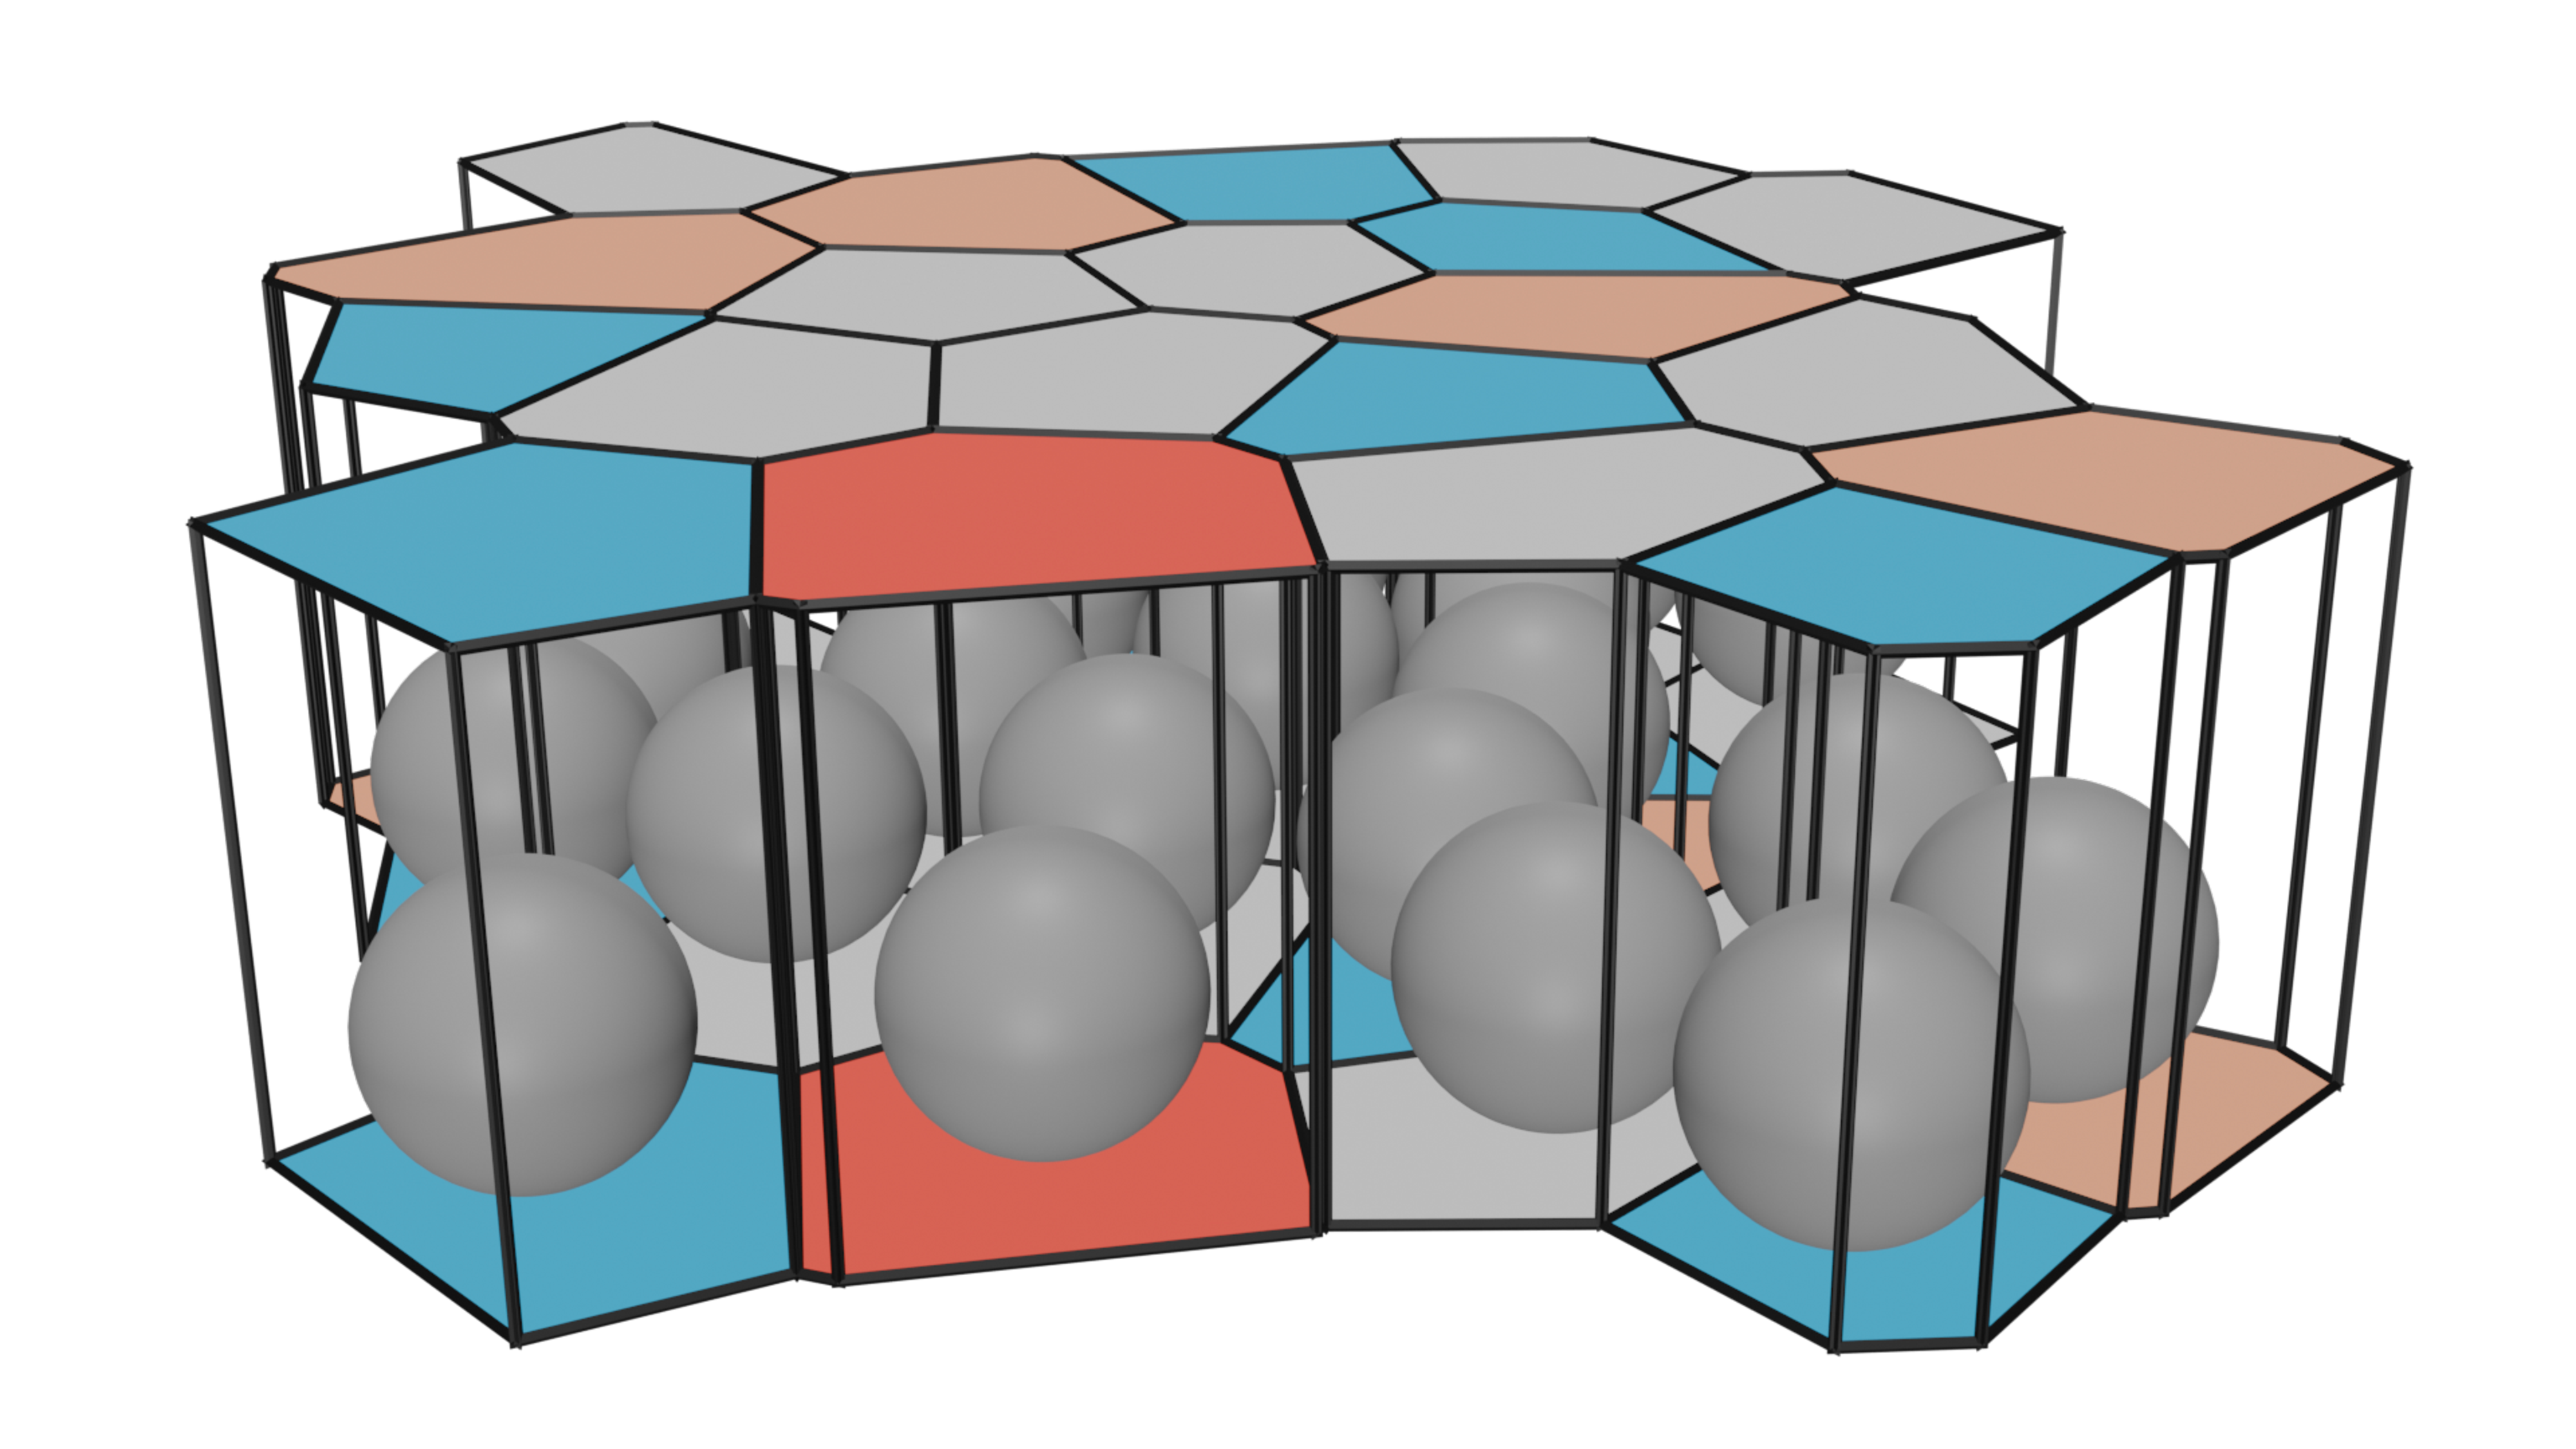
\includegraphics[width=\textwidth]{./figures/quasi2d/qtd_mono.pdf}
         \caption{}
         \label{fig:qtdv1}
     \end{subfigure}
     \hfill
     \begin{subfigure}[b]{0.45\textwidth}
         \centering
         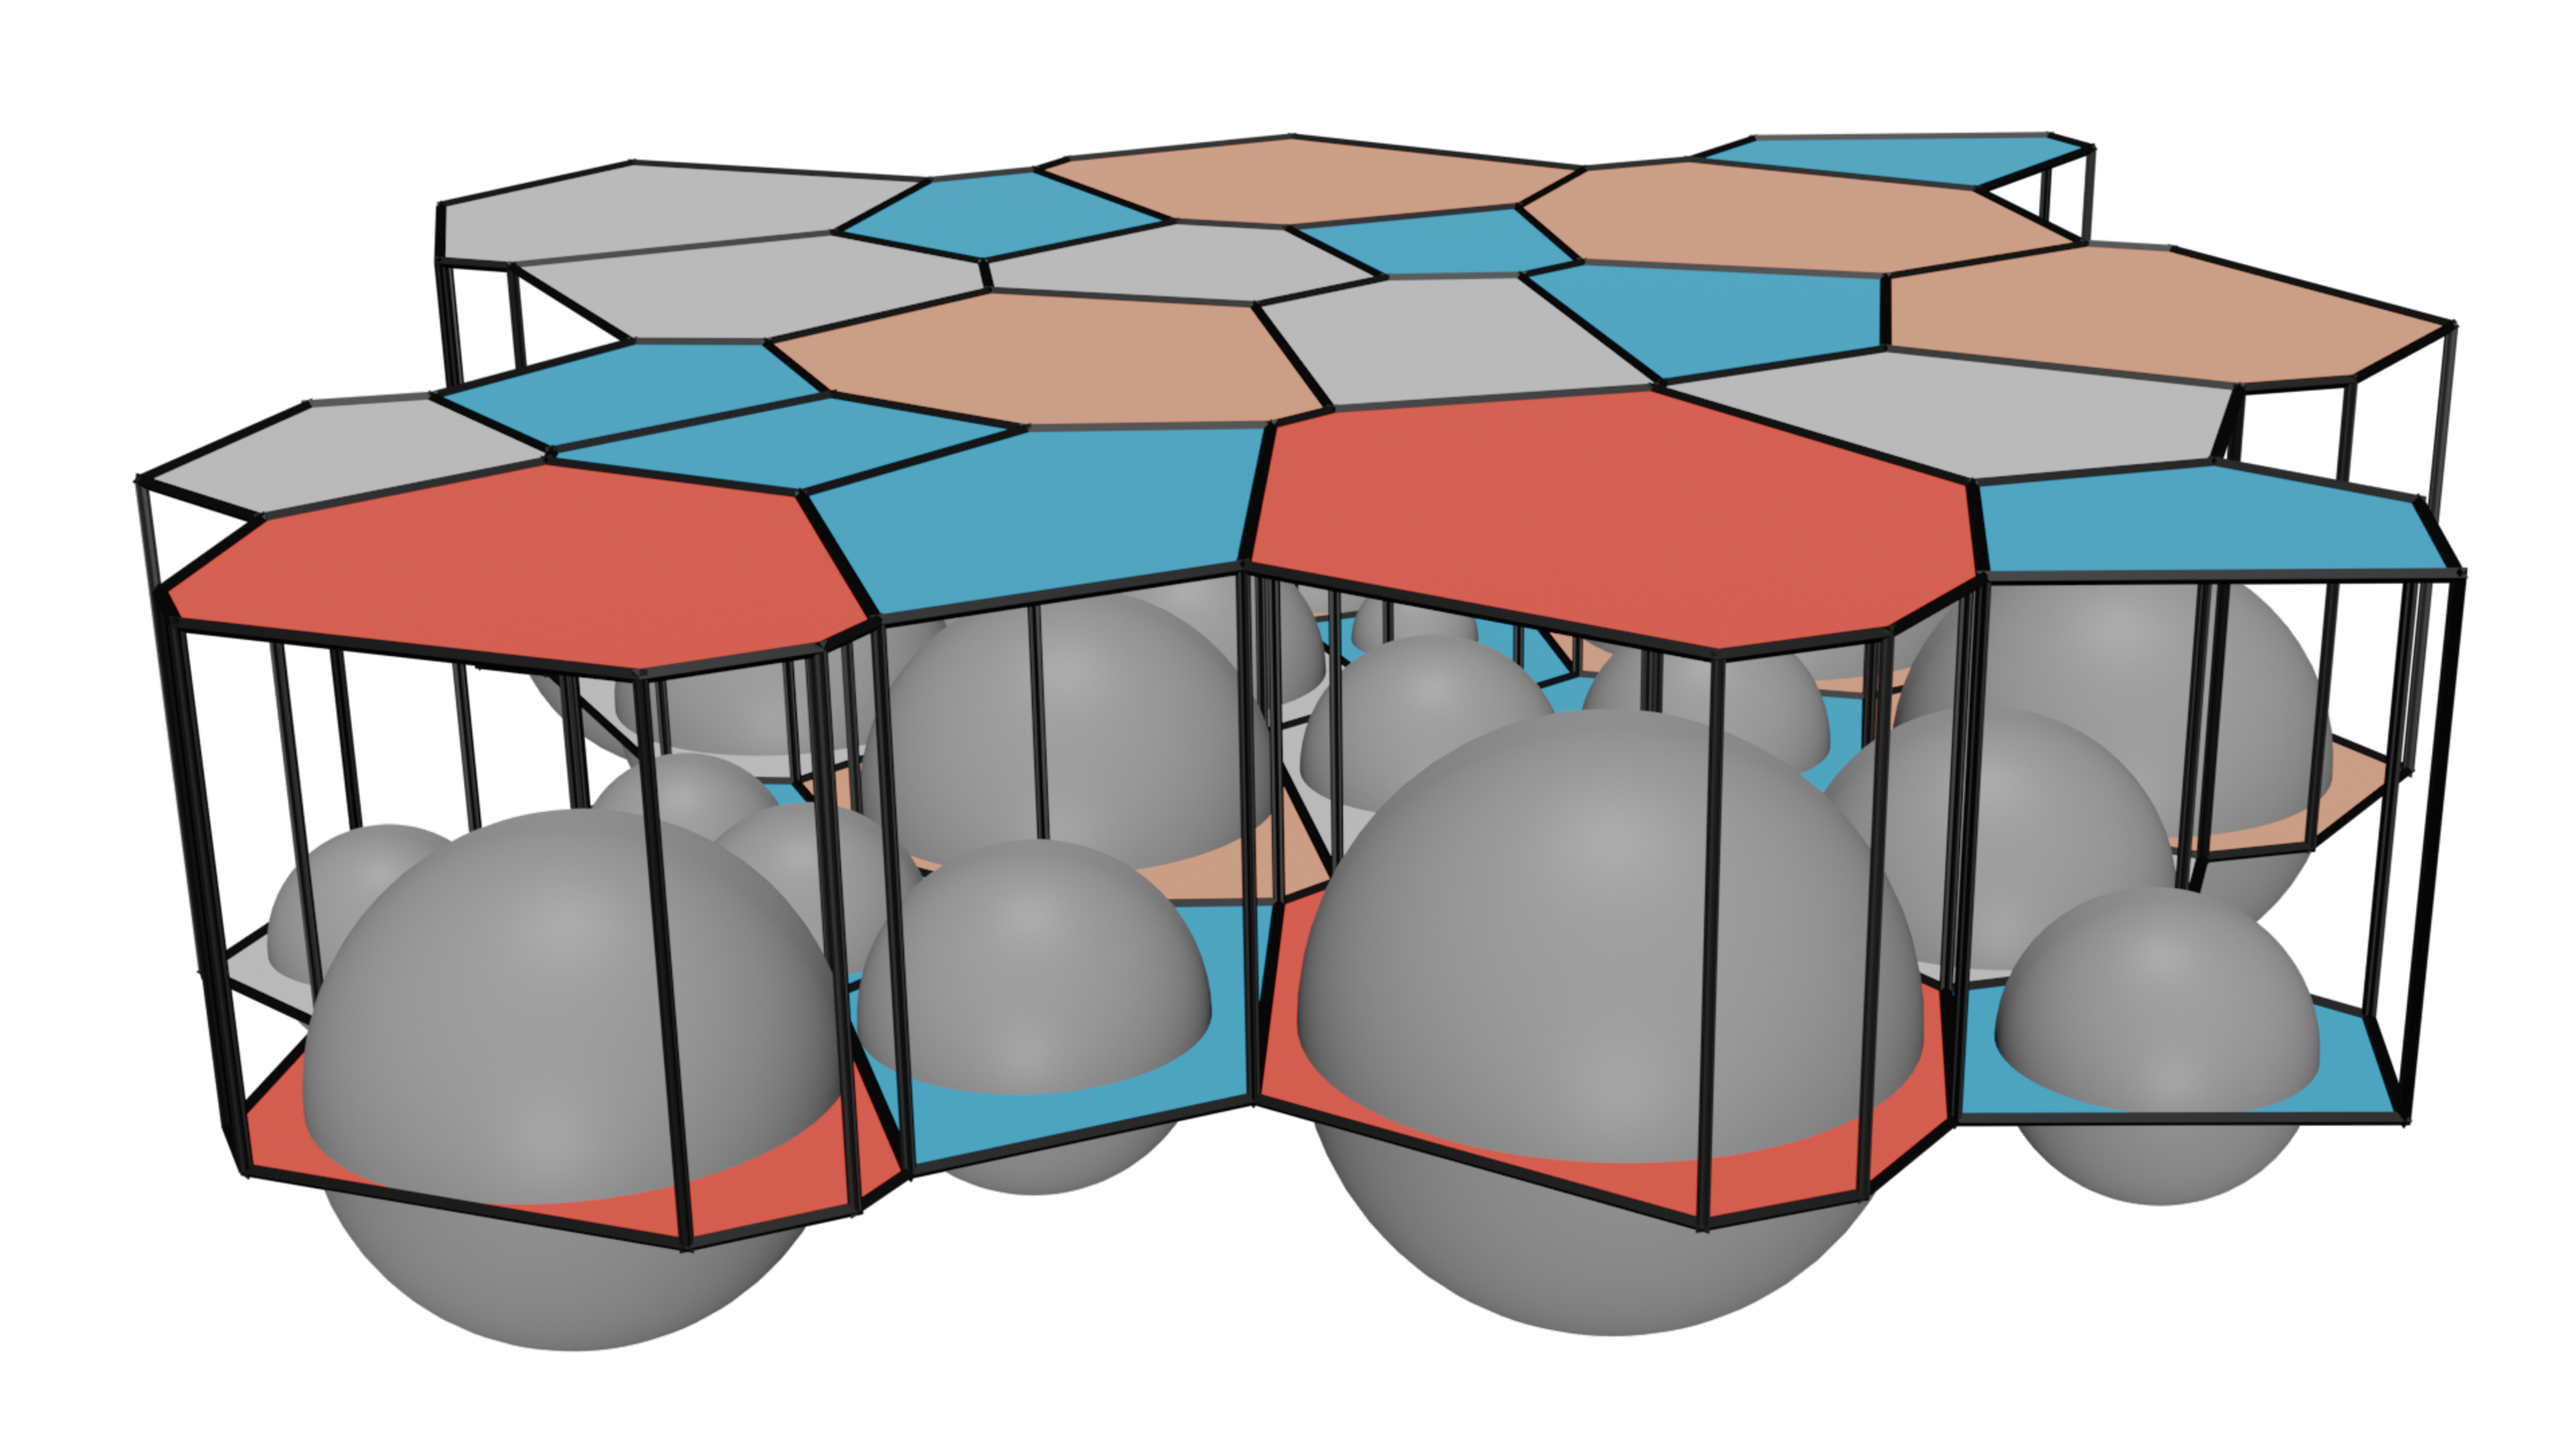
\includegraphics[width=\textwidth]{./figures/quasi2d/qtd_poly_add.pdf}
         \caption{}
         \label{fig:qtdv2}
     \end{subfigure}
     \hfill
     
     \begin{subfigure}[b]{0.45\textwidth}
         \centering
         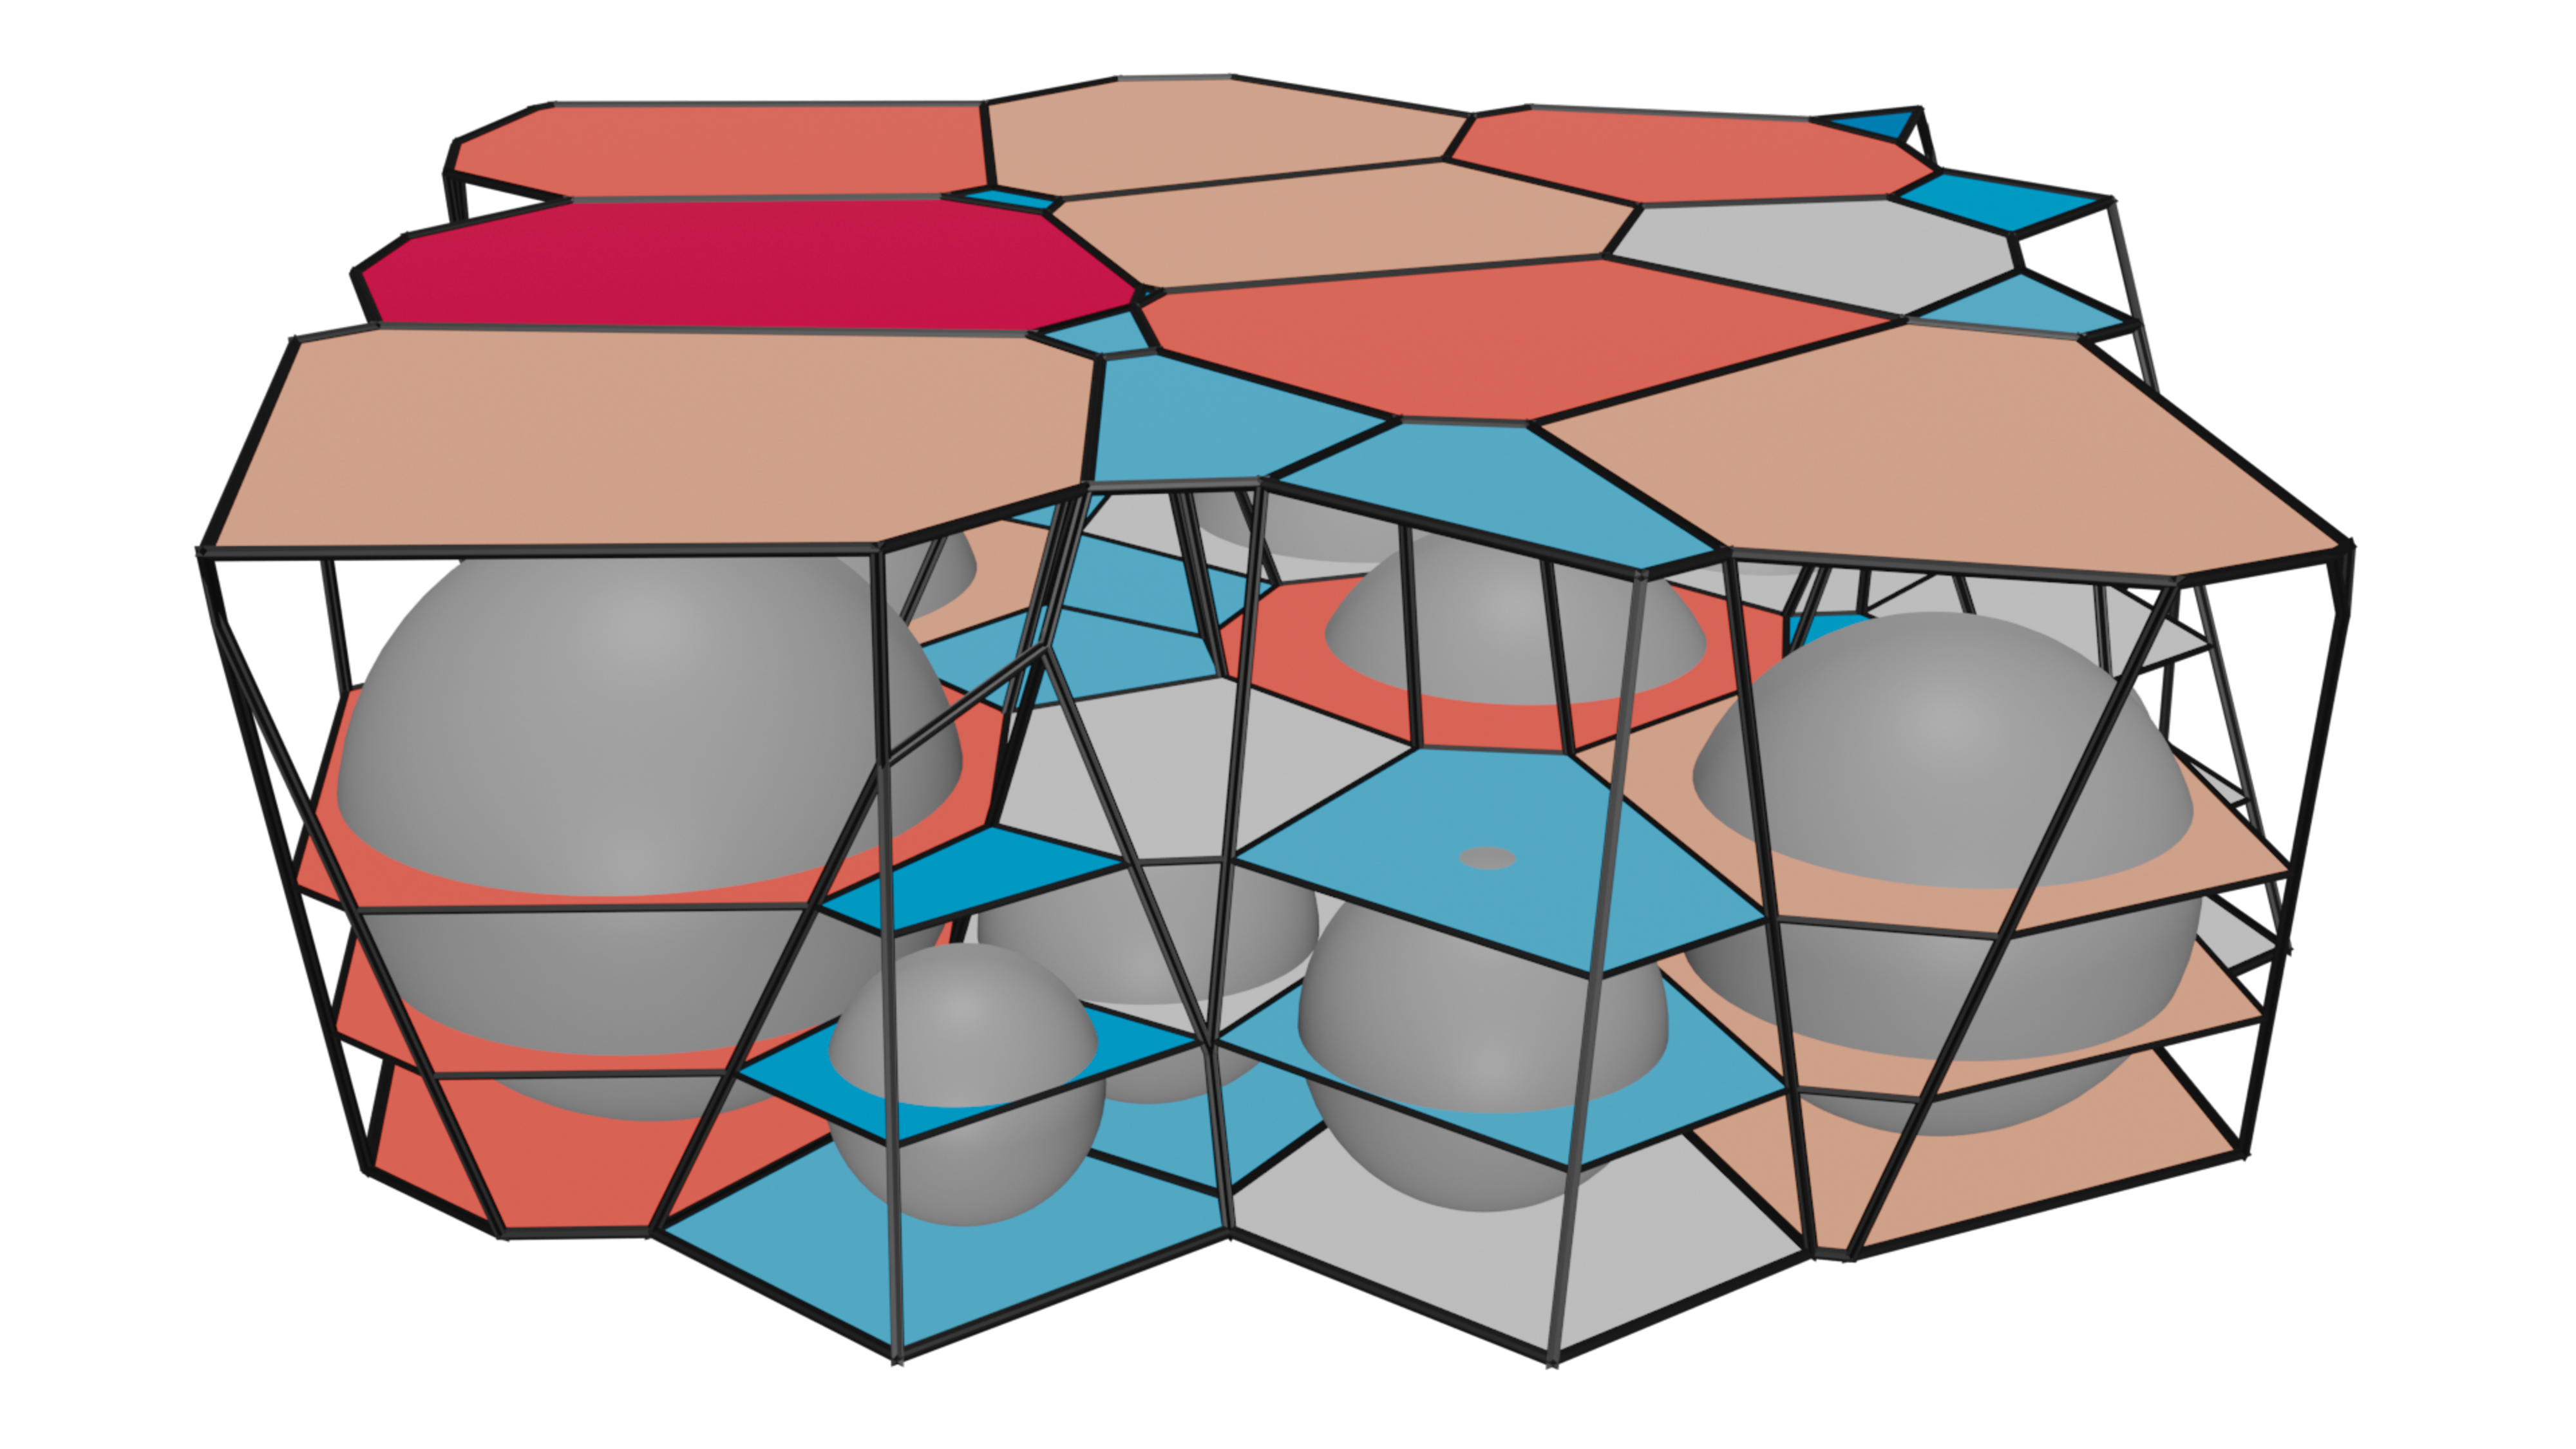
\includegraphics[width=\textwidth]{./figures/quasi2d/qtd_poly_nonadd.pdf}
         \caption{}
         \label{fig:qtdv3}
     \end{subfigure}
     \hfill
	
	
	\caption{Voronoi diagrams in three different quasi\--2D systems. The 3D Voronoi polyhedra are demarked by the thick black lines, whilst selected 2D Voronoi polygons are shaded. Panel (a) shows a monodisperse system with spheres sharing a basal plane and particle centres also occupying the same horizontal plane. Panel (b) shows a polydisperse system where particle centres lie in the same horizontal plane. A 3D Voronoi diagram weighted by the sphere radii is overlaid. Panel (c) shows a polydisperse system where particles share a basal plane. A 3D Voronoi diagram weighted by the sphere radii is overlaid.}
	\label{fig:qtdv}
\end{figure}

Various experimental approaches exist to create \qtd{} systems, including confining particles between two planes \cite{Marcus1997,Weikai2014}, adsorbed at an interface \cite{Peng2009,Vogel2014} as well as sedimentation on a surface \cite{Tamborini2015,Thorneywork2018}.
In fact, it is the nature of the system which will determine which Voronoi analysis is most appropriate.
Taking first the simplest \qtd{} case, of the monolayer of monodisperse spheres, the particle centres will occupy the same plane.
As demonstrated in figure \ref{fig:qtdv1}, the 3D Voronoi polyhedra for such system are prismatic, such that any horizontal cut through the construction will yield the same 2D tessellation. 
In addition, it is relatively straightforward to see that this 2D tessellation is topologically equivalent to the 2D Voronoi diagram, calculated in the plane of the particle centres.
This is to say that the 3D Voronoi can be trivially constructed from the 2D Voronoi, and so such systems can be analysed with an unweighted 2D Voronoi, with no loss of information.

A simple extension is then to take polydisperse particles in which the particle centres occupy the same plane (\eg{} particles suspended at an interface).
As previously alluded to, a weighted Voronoi construction is required in this case, to avoid the possibility of the polyhedra cutting through the larger particles.
Calculating the 3D Voronoi diagram, weighted by the sphere radii, once again leads to prismatic polyhedra, as shown in figure \ref{fig:qtdv2}.
Now the 2D tessellations formed from horizontal cuts are topologically equivalent to the 2D Voronoi diagram, weighted by the sphere radii, calculated in the plane of the particle centres.
Once again the partitioning of space can be fully described in two dimensions, and so such systems can be analysed with a weighted 2D Voronoi.

The more complex case is to consider a monolayer of polydisperse particles sedimented on a surface.
Under these conditions the spheres share a basal tangent plane, and the centres no longer occupy a common plane.
Although there is a trivial projection of the particle centres into 2D, the interaction distances between particles are non\--additive, reflecting the essential 3D nature of the problem.
As can be seen in figure \ref{fig:qtdv3}, the polyhedra in the 3D Voronoi diagram, weighted by sphere radii, are no longer prismatic.
The 2D tessellations formed from horizontal cuts through the system therefore have a non\--trivial relationship with cut height.
Rather, these 2D tessellations show an evolution in structure as the height above the basal plane increases - both in terms of the number of polygons and their properties.
Under these quasi\--2D conditions, it is not necessarily clear what is the best approach for conducting a Voronoi analysis, or even how to define even basic properties such as the packing fraction.

It is these final quasi\--2D systems which are the focus of this chapter.
In this section, it will be demonstrated that for these systems, the basal tessellation in the weighted 3D Voronoi is topologically equivalent to an unweighted 2D Voronoi diagram.
This result will be extended to explore the more general stereology problem, showing that tessellation at an arbitrary cut height above the basal 2D plane can be related to a 2D weighted Voronoi diagram.
These tessellations will also be compared to those formed from equivalent arrangements of hard disks.

\davidnote{Revisit Voronoi section in methods.}

\subsection{Polydisperse Hard Sphere Model}

As a generalisation, this section now considers a system of polydisperse hard spheres sedimented onto a surface, such that all spheres share a common basal tangent plane.
For numerical simulations, it will further be constrained that the radii, $\rs_i$, of the particles follow a lognormal distribution:
\begin{equation}
	\label{eq:lognormal}
	f\left(\rs\right)=\frac{1}{\rs\sqrt{2\pi\sigma^2}}\exp{\left[-\left(\frac{\ln{\rs}-\mu}{\sqrt{2\sigma^2}}\right)^2\right]}\,,
\end{equation}
where as usual $\mu$ and $\sigma$ are respectively the mean and standard deviation of the logarithm of the radii.
This distribution is chosen to ensure the radii of randomly generated particles are always positive.
Whilst the choice of distribution does not affect the fundamental conclusions of the Voronoi analysis below, it will help quantify properties of the system such as the packing fraction.

\subsection{Stereological Relationships}
\label{sec:vorrel}

The unweighted and weighted Voronoi constructions were introduced in section \ref{s:voronoiintro}.
To review, the unweighed Voronoi requires only the positions of the particle centres, placing dividing planes halfway between neighbouring points.
The weighted radical variant requires knowledge of both positions and radii of the particles, repositioning the dividing planes further from the larger particles, hence allocating more them more space.
When studying \qtd{} colloids, it is possible to construct a 3D weighted Voronoi using the coordinates of the particle centres, $\mathbf{r}_i=\left(x_i,y_i,\rs_i\right)$.
However, in most cases researchers prefer to analyse configurations using a 2D Voronoi using the projected particle centres $\mathbf{r}_i^\prime=\left(x_i,y_i\right)$. 
The rational behind this is clear: 2D analysis is easier to visualise and rationalise.
In addition, as in figure \ref{fig:qtdv1}, for monodisperse systems the 3D representation contains no more information on neighbouring interactions and assigned volumes than the 2D analogue.
However, as in figure \ref{fig:qtdv3}, for polydisperse particles whilst this may be a good first approximation, this is not necessarily accurate, and so it is important to examine the relationship between Voronoi diagrams in two and three dimensions to ensure correct physical meaning is attributed to the Voronoi analysis.

\subsubsection{Limiting Case with Basal Plane}

To begin with, the stereological relationship between the 3D weighted Voronoi and the 2D tessellation formed from the intersection of the radical planes with the basal tangent plane will be considered.
In figure \ref{fig:qtdv3}, this corresponds to the bottommost 2D tessellation.
To do this, take the arrangement in figure \ref{fig:qtdda}, with two spheres $A$,$B$ separated by the dividing radical plane, $V$, and sharing the tangent plane, $T$, with equation $z=0$.
The distance between the sphere centres is $r_{AB}$, whilst the distance between the projected centres is denoted $r_{AB}^\prime$.
The dividing plane $V$, has a normal given by $\mathbf{n} =\overrightarrow{AB}=r_{AB}^\prime\boldsymbol{\hat{\textbf{\i}}}+\left(\rs_B-\rs_A\right)\mathbf{\hat{k}}$.
In addition the point $D$ which lies on $V$ is located at $\overrightarrow{OD}=d_{A}\mathbf{\hat{n}}+\rs_A\mathbf{\hat{k}}$ where $d_{A}=\frac{\rs_A^2-\rs_B^2+r_{AB}^2}{2r_{AB}}$ and $\abs{\mathbf{n}}=r_{AB}$.
Defining the direction of $x$ as as the projection of $d_A\mathbf{\hat{n}}$ on the basal plane, the plane equation for $V$ can be deduced as:
\begin{equation}
	\label{eq:plane}
	r_{AB}^\prime x+\left(\rs_B-\rs_A\right)z=\frac{\left(r_{AB}^\prime\right)^2}{2}\,.
\end{equation}
The intersection of $V$ with $T$ occurs at $z=0$, and so the line of intersection is given simply by $x=r_{AB}^\prime/2$.
However there is something significant about this result: this dividing line in 2D is the same as that which would be obtained from constructing the 2D unweighted Voronoi using the projected particle centres $\mathbf{r}^\prime_i$.
As this must be true for all pairs of neighbouring particles, it follows that the entire 2D unweighted Voronoi will be constructed. 
This leads to the key relationship of this work: for quasi\--2D systems of spheres, the unweighted 2D Voronoi diagram is topologically equivalent to the tessellation formed by taking the basal faces of the polyhedra in the weighted 3D Voronoi diagram. 
This holds when the 2D Voronoi is constructed using the point set of the sphere centres projected onto the basal plane, and the 3D Voronoi using the point set of the original sphere centres and weighted by the sphere radii.

\begin{figure}[tb]
	\centering
     
      \begin{subfigure}[b]{0.40\textwidth}
         \centering
         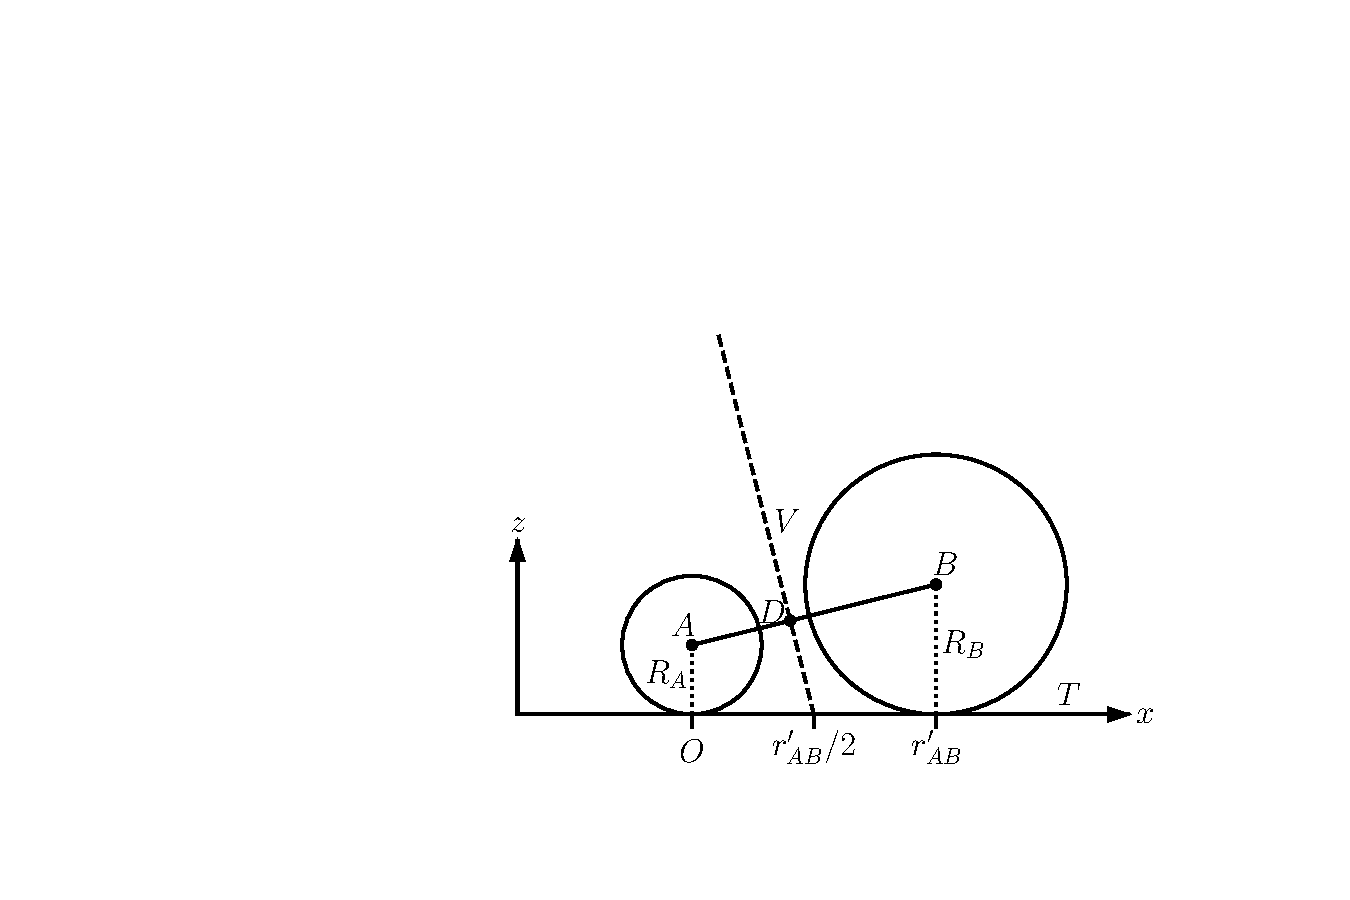
\includegraphics[width=\textwidth]{./figures/quasi2d/qtd_dia_a.pdf}
         \caption{}
         \label{fig:qtdda}
     \end{subfigure}
     \hfill
     
     \begin{subfigure}[b]{0.48\textwidth}
         \centering
         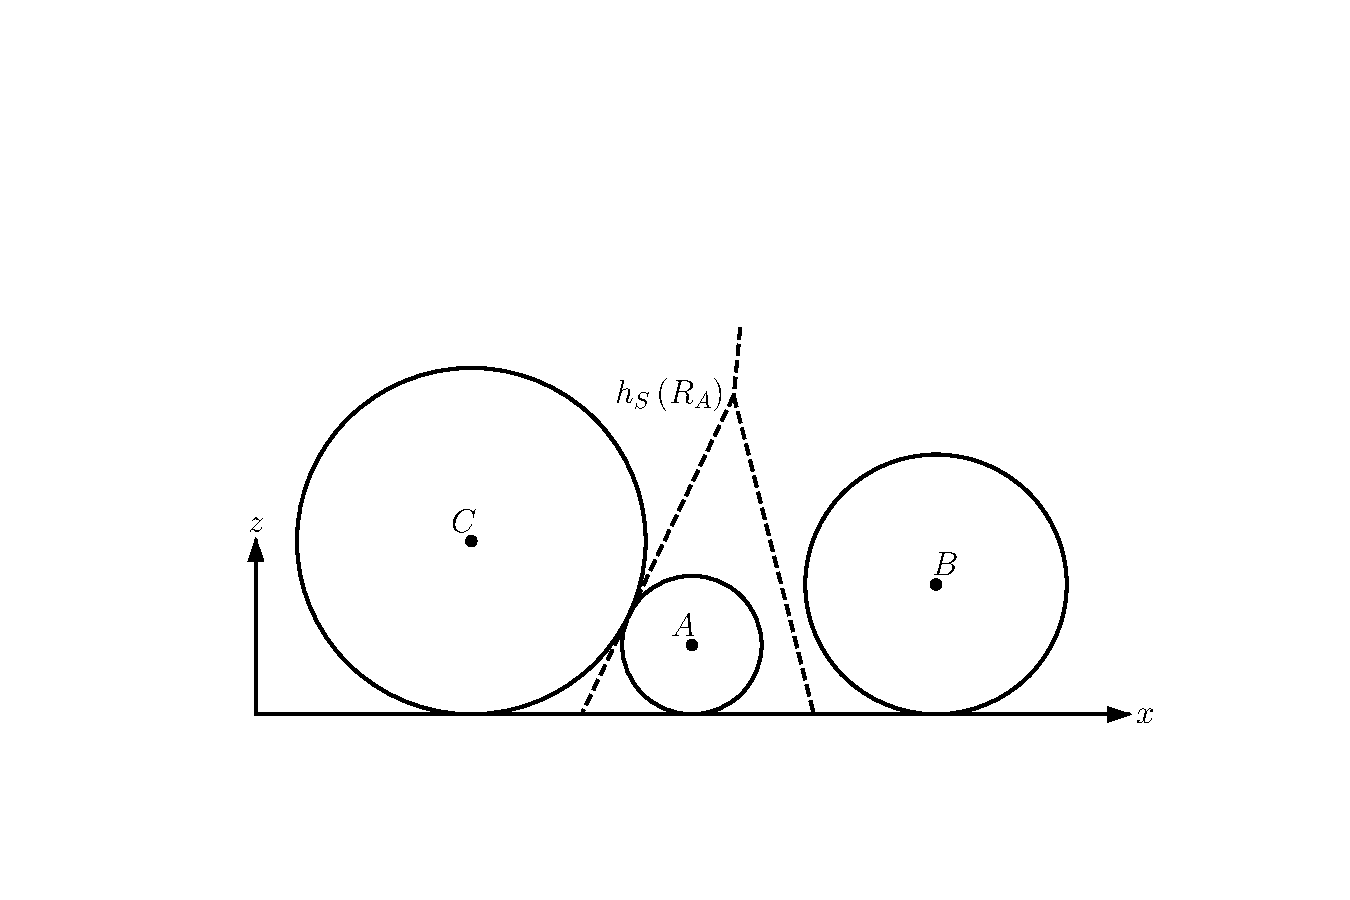
\includegraphics[width=\textwidth]{./figures/quasi2d/qtd_dia_b.pdf}
         \caption{}
         \label{fig:qtddb}
     \end{subfigure}
     \hfill
     \begin{subfigure}[b]{0.48\textwidth}
         \centering
         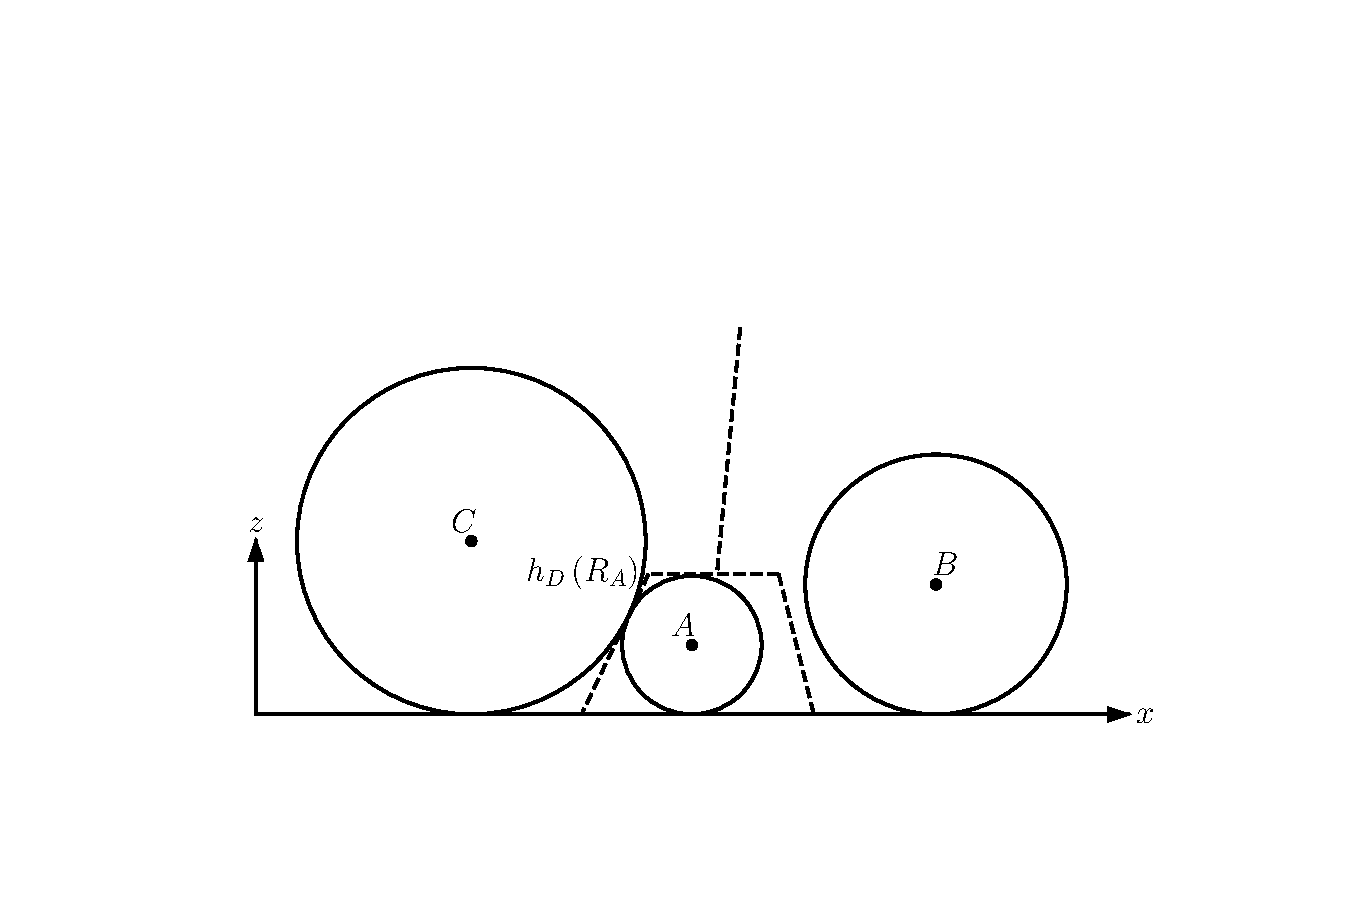
\includegraphics[width=\textwidth]{./figures/quasi2d/qtd_dia_c.pdf}
         \caption{}
         \label{fig:qtddc}
     \end{subfigure}
     
     	\caption{Panel (a) shows two spheres and the dividing radical plane between them. The radical plane intersects the tangent plane at half the horizontal distance between the particles. This intersection generates the same dividing line in the tangent plane as would the unweighted Voronoi using the projected particle positions.
Panel (b) shows three spheres and the 3D weighted Voronoi polyhedron formed around sphere $A$. The height of the cell is given by the topmost point, denoted $h_S\left(R_A\right)$. Panel (c) shows the same three spheres and the polyhedron that would be formed from stacking 2D Voronoi tessellations with disk radii as weights. As the weight for $A$ is not defined above the sphere diameter, the polyhedron is truncated in comparison with in panel (b). The height of the cell is then given by $h_D\left(R_A\right)=2R_A$.}
	\label{fig:qtdd}
\end{figure}

\subsubsection{General Case with Arbitrary Horizontal Plane}

Taking the basal faces of the 3D Voronoi polyhedra can equally be thought of as taking a horizontal cut through the tessellation at $z=0$.
The result above is essentially a special case of the fact that a cut through a 3D Voronoi must yield a tessellation which is equivalent to some weighted 2D Voronoi \cite{Imai1985,Rivier1990}.
Following from the result above, one may ask what is the analogous relationship between a 2D and 3D Voronoi when taking a cut at arbitrary $z$, as in figure \ref{fig:qtdv3}.
Revisiting the simple arrangement in figure \ref{fig:qtdda}, for a given horizontal cut height, $z$, the projected particle centres are now defined as $\mathbf{r}_i^\prime=\left(x_i,y_i,z\right)$.
Regardless of the the value of $z$, we note that the distances between the projected centres remain the same at $r_{AB}^\prime$.
To obtain the same distance between the projected particle centres and the dividing plane using both a 2D and 3D Voronoi, it can be seen from combining equations \eqref{eq:radical} and \eqref{eq:plane} that:
\begin{equation}
	\label{eq:condition}
	w_A^2-2\rs_Az = w_B^2-2\rs_Bz\,.
\end{equation}
The simplest solution for the weights that satisfy this equation is therefore:
\begin{equation}
	\label{eq:mapweights}
	w_{S,i} = \left(2\rs_iz\right)^{1/2}\,.
\end{equation}
Again as this will naturally extend to a collection of many spheres, a more general relationship is obtained: for quasi\--2D systems of spheres, the tessellation formed from a horizontal cut through a 3D Voronoi diagram weighted by the sphere radii, is topologically equivalent to a 2D Voronoi diagram weighted according to equation \eqref{eq:mapweights}.
This holds when the 3D Voronoi is constructed using the point set of the original sphere centres, and the 2D Voronoi using the point set of the sphere centres projected onto the horozontal cut plane. 
The caveat to this result is that if the cut is height is greater than the maximum cell height for a given sphere, such a sphere must be excluded from the 2D Voronoi calculation.
Moreover, the key result in the above section is simply a limiting case of this more general result, when $z = 0$ and the weights are trivially zero. 
In addition, in the limiting case, it follows that all spheres must have a cell in the 2D Voronoi.
This 2D weighted Voronoi diagram shall be referred to as the sphere\--weighted Voronoi and variables associated with it denoted with a subscript $S$.

\subsubsection{Connection to System of Hard Disks}

A horizontal cut through a 3D system of hard spheres will produce a 2D system of hard disks.
The radii of these disks will be related to the radii of the spheres, and if they are used as weights in a 2D Voronoi analysis they will also satisfy equation \eqref{eq:condition}:
\begin{equation}
	\label{eq:radii}
	w_{D,i}  = \left(2\rs_i z-z^2\right)^{1/2}\,.
\end{equation}
This suggests that the tessellation formed from the horizontal cut through the 3D Voronoi should also be equivalent to the 2D Voronoi using these disk radii.

However, there is a caveat to this result. 
It is clear that equation \eqref{eq:radii} is only well defined for $z\leq 2\rs_i$ \ie{} the cut height is less than the sphere diameter.
There is no such constraint for the polyhedral cells in the 3D weighted Voronoi, which may readily extend above the associated particle.
Therefore, the result above is only strictly true when the cut height is less than the smallest sphere diameter.
A modification is made where points which have diameters less than the cut height are excluded from the 2D calculation.
These excluded particles will therefore not have cells in the Voronoi tessellation.
In this case some 3D cells will become truncated in the 2D representation, as shown in figures \ref{fig:qtddb} and \ref{fig:qtddc}.
This will lead to an increasing difference between the two types of partitions as the cut height is increased, as demonstrated in figure \ref{fig:vorcuts}.
This 2D weighted diagram shall be referred to as the disk\--weighted Voronoi and variables associated with it denoted with a subscript $D$.

\begin{figure}[tb]
	\centering
     
      \begin{subfigure}[b]{0.23\textwidth}
         \centering
         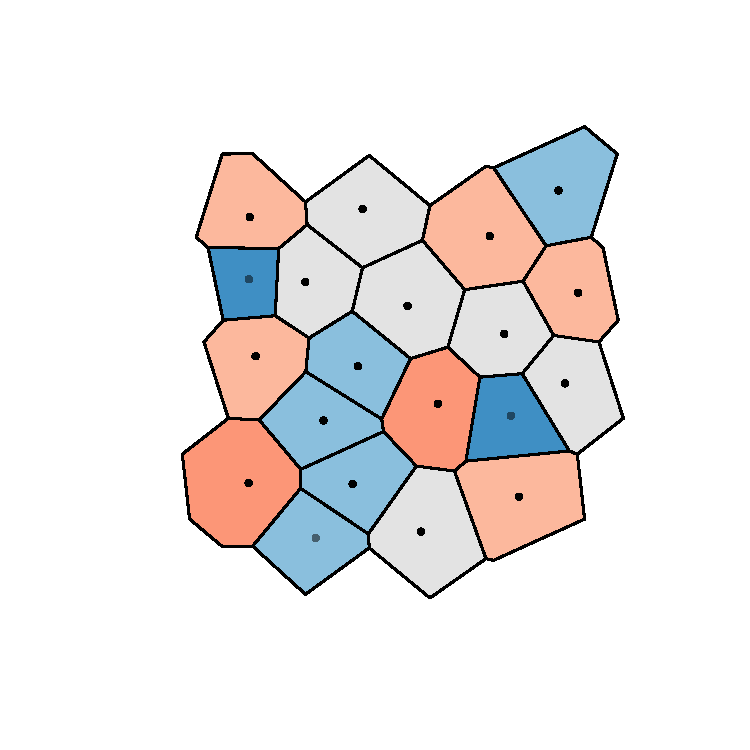
\includegraphics[width=\textwidth]{./figures/quasi2d/cut_z0_a.pdf}
         \caption{Sphere weighted, \\$z=0$.}
         \label{fig:cut0a}
     \end{subfigure}
     \hfill
      \begin{subfigure}[b]{0.23\textwidth}
         \centering
         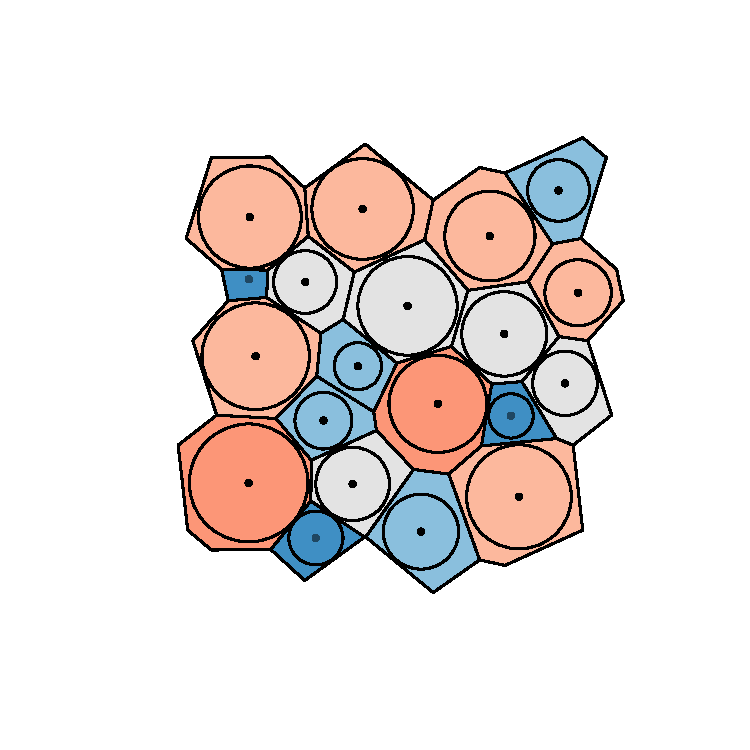
\includegraphics[width=\textwidth]{./figures/quasi2d/cut_z10_a.pdf}
         \caption{Sphere weighted, \\$z=1$.}
         \label{fig:cut10a}
     \end{subfigure}
     \hfill
      \begin{subfigure}[b]{0.23\textwidth}
         \centering
         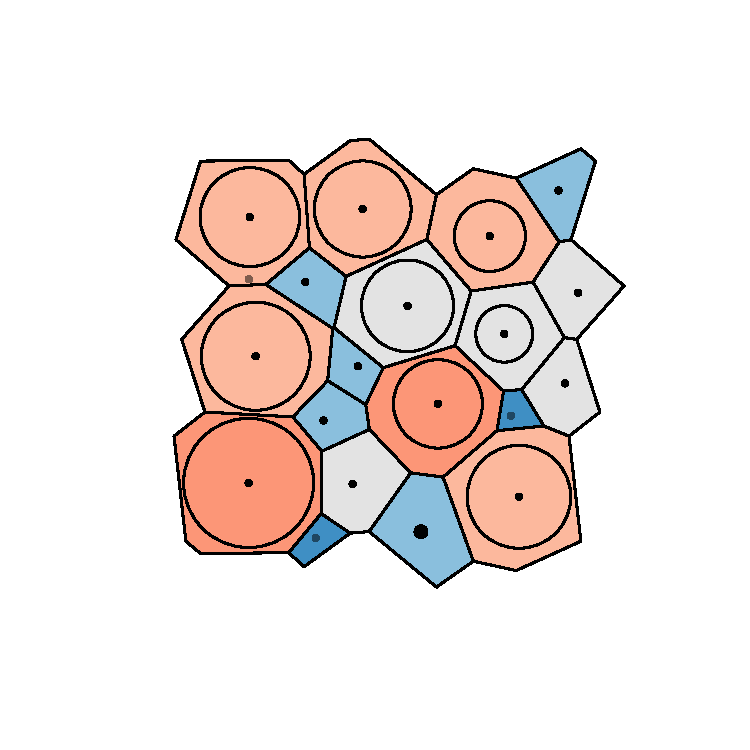
\includegraphics[width=\textwidth]{./figures/quasi2d/cut_z20_a.pdf}
         \caption{Sphere weighted, \\$z=2$.}
         \label{fig:cut20a}
     \end{subfigure}
     \hfill
      \begin{subfigure}[b]{0.23\textwidth}
         \centering
         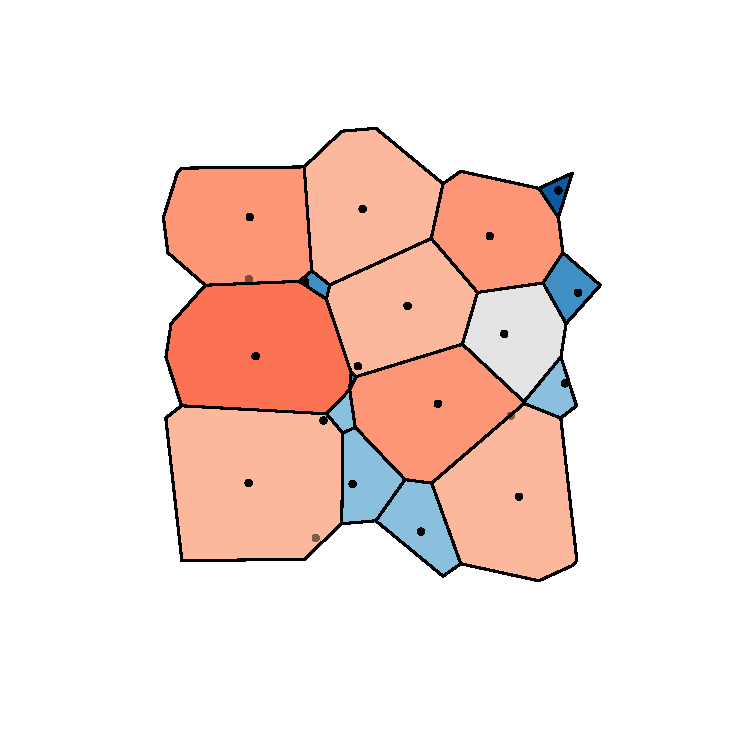
\includegraphics[width=\textwidth]{./figures/quasi2d/cut_z40_a.pdf}
         \caption{Sphere weighted, \\$z=4$.}
         \label{fig:cut40a}
     \end{subfigure}
     \hfill
     \vspace{0.5cm}
     
      \begin{subfigure}[b]{0.23\textwidth}
         \centering
         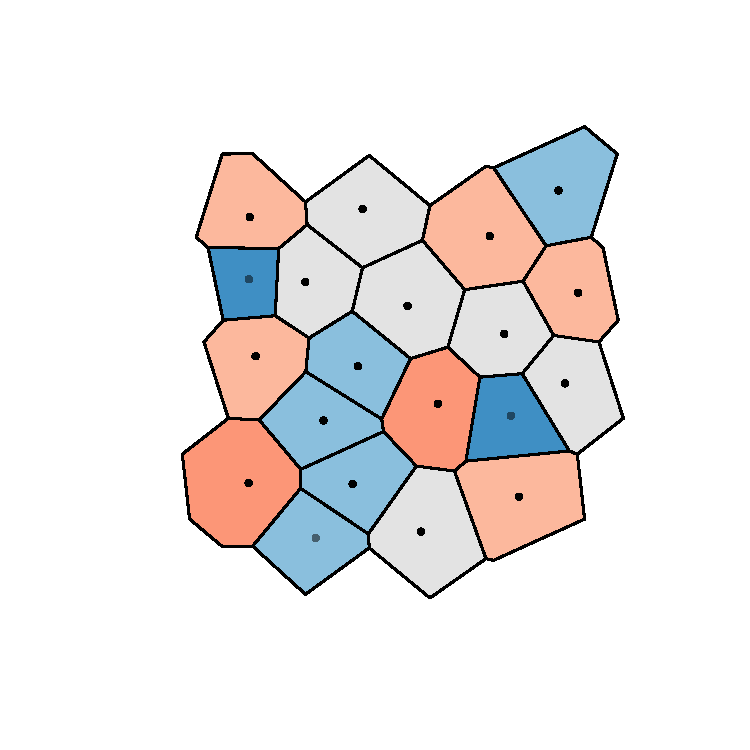
\includegraphics[width=\textwidth]{./figures/quasi2d/cut_z0_b.pdf}
         \caption{Disk weighted, \\$z=0$.}
         \label{fig:cut0b}
     \end{subfigure}
     \hfill
      \begin{subfigure}[b]{0.23\textwidth}
         \centering
         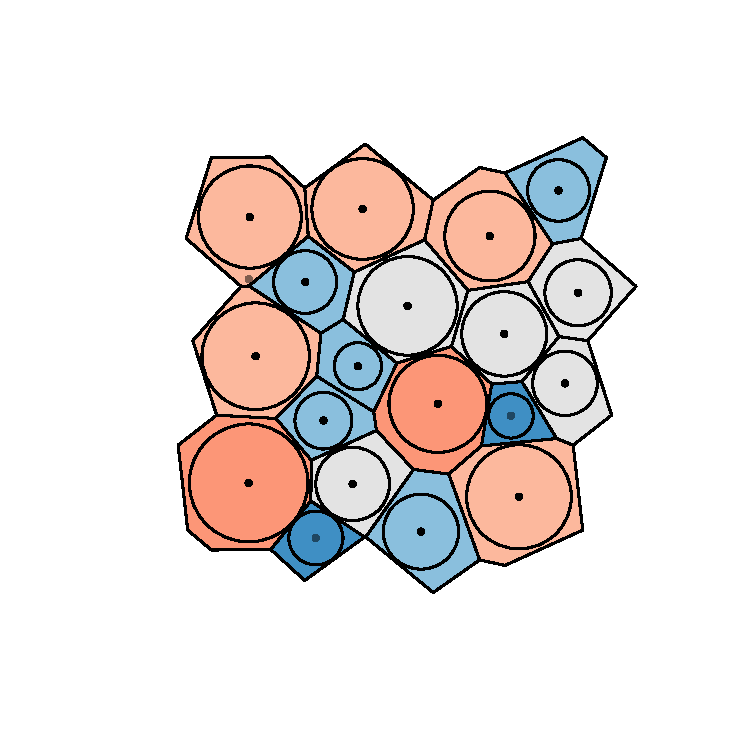
\includegraphics[width=\textwidth]{./figures/quasi2d/cut_z10_b.pdf}
         \caption{Disk weighted, \\$z=1$.}
         \label{fig:cut10b}
     \end{subfigure}
     \hfill
      \begin{subfigure}[b]{0.23\textwidth}
         \centering
         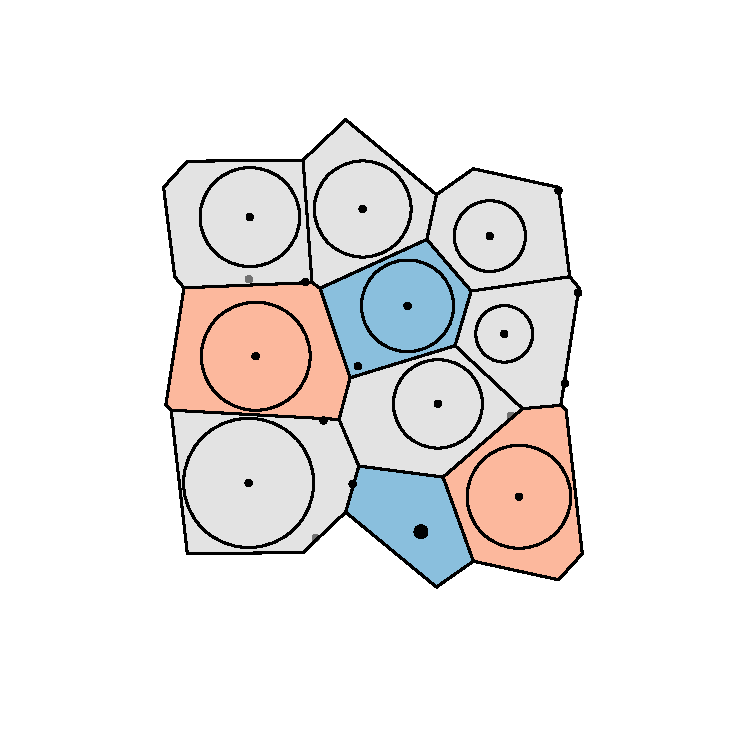
\includegraphics[width=\textwidth]{./figures/quasi2d/cut_z20_b.pdf}
         \caption{Disk weighted, \\$z=2$.}
         \label{fig:cut20b}
     \end{subfigure}
     \hfill
     \begin{subfigure}[b]{0.23\textwidth}
         \centering
         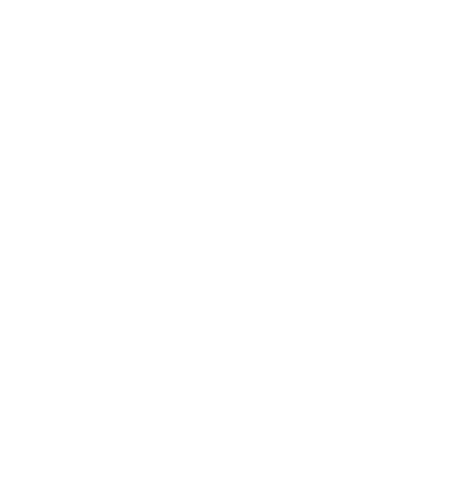
\includegraphics[width=\textwidth]{./figures/quasi2d/empty.pdf}
     \end{subfigure}
     
\caption{Comparison of the tessellations formed from a horizontal cut through a 3D Voronoi diagram weighted by sphere radii (a)-(d) and a 2D Voronoi diagram weighted by disk radii (e)-(g), at increasing $z$ values.
	The same configuration is used as in figure \ref{fig:qtdv3}, with the horizontal cuts corresponding to the left hand diagrams.
	Black circles indicate the particle radii at the cut height, which also correspond to the weights in the disk\--weighted Voronoi. Black points indicate the projected particle centres, whilst grey points indicate particles without corresponding cells in the 2D tessellation.}
	\label{fig:vorcuts}
\end{figure}

\subsection{Properties of Voronoi Tessellations}

The important properties of the sphere and disk\--weighted Voronoi diagrams are outlined in this section, which will aid with their analyses.
These include the expected number of points at a given cut height, the weight distribution of the included points and the nearest\--neighbour distances between them.
These are the quantities that appear in equation \eqref{eq:radical} and therefore govern the wider properties of the Voronoi diagram. 
The analytic results will be demonstrated for the model of lognormally distributed sphere radii will, but the results extend to any configuration where the sphere radii are known.

\subsubsection{Average Nearest\--Neighbour Distances}

A useful metric is the expected distance between points in a Voronoi diagram at different cut heights, as this can be used to rationalise much of the observed behaviour.
In order to do this, it is necessary to assume that particles are uniformly distributed (the ideal gas), neglecting the short range liquid structure.
Whilst this might seem an over\--simplification, not only does the approximation get better at lower packing fractions but also as the cut height is increased, particles are lost from the tessellation and their positions become effectively decorrelated. 

Firstly, the average distance between all points in neighbouring Voronoi cells at a given cut height, $\ed$, can be found as follows.
The number density at a given cut height, denoted $\rho_z$, is introduced as the number of points at height $z$, divided by the total area of the 2D Voronoi diagram.
It can therefore be expressed:
\begin{equation}
	\label{eq:numden}
	\rho_z = \rho_0 \zN\,,
\end{equation}
where $\rho_0$ is the number density considering all points (as must be the case at $z=0$), and $N\left(z\right)$ is the proportion of particles included at a given cut height.
By dividing the area equally between all particles, we expect the average distance between neighbouring points in the 2D Voronoi diagram to follow:
\begin{equation}
	\label{eq:ndist}
	\ed = 2\left(\frac{1}{\pi\rho_z}\right)^{1/2}.%=2\left(\frac{1}{\pi\rho_0\zN}\right)^{1/2}\,.
\end{equation}

Alternatively, one can opt to find the average distance to the $n^{\mathrm{th}}$ nearest neighbour, $\edn$.
If again a uniform distribution of spheres is assumed (\ie{} the dilute limit), Bhattacharyya and Chakrabarti \cite{Bhattacharyya2008}, showed that in two dimensions, this is given by the equation:
\begin{equation}
	\label{eq:nndist}
	\edn = \left(\frac{1}{\pi\rho_z}\right)^{1/2}\frac{\Gamma{\left(n+1/2\right)}}{\Gamma{\left(n\right)}}\,.
\end{equation}

\subsubsection{Properties of Disk\--Weighted Voronoi}

The properties of the disk\--weighted Voronoi are somewhat easier to see and so it is logical to begin with these.
The height below which a Voronoi cell is defined for a particle of a certain radius is given exactly by $h_D\left(R\right)=2R$, as in figure \ref{fig:qtddc}.
Hence, for a given cut height, the particles with associated cells in the tessellation will be all those with radii in excess of the inverse function $h_D^{-1}\left(z\right)=z/2$.
The proportion of particles with associated cells above a given cut height, denoted $\nDz$, is therefore related to the cumulative distribution function of the sphere radii:
\begin{equation}
	\label{eq:ndz}
	\nDz = \int_{z/2}^\infty f\left(\rs\right) \dd\rs = \frac{1}{2}\text{erfc}\left[\frac{\ln{\left(z/2\right)}-\mu}{\sqrt{2\sigma^2}}\right]\,,
\end{equation}
as all particles with $R < z/2$ are neglected.

The moments of the weight distribution function at a given cut height can then be calculated by integrating over the range of the remaining particle radii,
\begin{equation}
	\label{eq:wmom}
	\ewDn = \frac{1}{\nDz}\int_{z/2}^\infty  \left(2Rz-z^2\right)^{n/2} f\left(R\right) \dd R\,.
\end{equation}
as required.
For example, the analytic solution for the second moment can be found in section \ref{s:qtdpackingfrac}.

\subsubsection{Properties of Sphere\--Weighted Voronoi}

For the sphere\--weighted Voronoi, the maximum height of the Voronoi cell for a particle of a certain radius, $h_S\left(R\right)$, is not precisely defined with $R$.
Instead an approximate form will be derived below.
Regardless of the functional form of $h_S\left(R\right)$, in a similar manner to above an equation can be written for the proportion of particles with associated cells above a given cut height, denoted $\nSz$, as:
\begin{equation}
	\label{eq:nsz}
	\nSz = \int_{h_{S}^{-1}\left(z\right)}^\infty f\left(\rs\right) \dd\rs = \frac{1}{2}\text{erfc}\left[\frac{\ln{\left(h_{S}^{-1}\left(z\right)\right)}-\mu}{\sqrt{2\sigma^2}}\right]\,,
\end{equation}
with the moments of the weights at a given cut height provided by:
\begin{equation}
	\label{eq:wns}
	\ewSn = \frac{1}{\nSz}\int_{h_{S}^{-1}}^\infty  \left(2Rz\right)^{n/2} f\left(R\right) \dd R\,,
\end{equation}
in analogy with the disk\--weighted case.

The functional form of $h_S\left(R\right)$ can now be considered.
Rather than an exact relationship, an expression for the expected Voronoi cell height for a given particle radius is proposed.
The height of a Voronoi cell is a complex function that must depend on both the radius of the associated particle and the distances to neighbouring particles. 
In the following arguments it will be useful to refer to figures \ref{fig:qtdv}, \ref{fig:qtdd} and \ref{fig:vorcuts}.
Consider a reference particle of a given radius, $R^\prime$.
Crucially, the dividing planes forming the Voronoi polyhedron around it will only converge to a point when the neighbouring particles are larger than the reference particle.
For the purposes of this analysis, one can therefore think of the particle operating in a reduced density system containing only the particles with radii greater of equal to the reference particle.
The density is therefore,
\begin{equation}
	\label{eq:rhoref}
	\rho^\prime = \rho_0 \int_{R^\prime}^{\infty} f\left(R\right) \dd R\,,
\end{equation}
and mean average particle radius,
\begin{equation}
	\langle R^\prime \rangle = \frac{\int_{R^\prime}^{\infty} R f\left(R\right) \dd R }{\int_{R^\prime}^{\infty} f\left(R\right) \dd R}\,.
\end{equation}
In addition, the average $n^{\mathrm{th}}$ nearest neighbour distance will be given by equation \eqref{eq:nndist}, substituting the density from equation \eqref{eq:rhoref} above.

Therefore the average environment around the reference particle can be considered to consist of particles with radii $\langle R^\prime \rangle$ at located at successive distances $\langle d^\prime_n\rangle$.
These particles will generate dividing Voronoi planes according to equation \eqref{eq:plane}.
If it is then assumed that, on average, the highest point in the Voronoi polyhedron will occur above the particle centre (\ie{} $x=0$, see for example the cells in figure \ref{fig:qtdv}), the expected maximum cell height can be approximated by:
\begin{equation}
	h_{S,n}\left(R^\prime\right) \sim \frac{\langle r^\prime_n\rangle^2}{2\left(\langle R^\prime \rangle - R^\prime\right)}\,.
\end{equation}
These can be averaged over $m$ nearest neighbours to give the result:
\begin{equation}
	h_S\left(R^\prime\right) = \frac{1}{2m\left(\langle R^\prime\rangle-R^\prime\right)}\sum\limits_{n=1}^{m} \langle r^\prime_n \rangle^2\,.
\end{equation} 
It will be shown in section \ref{s:polycell} and figure \ref{fig:nphi}, that averaging over $m=3$ nearest neighbour distances gave a good fit to the observed numerical distribution.
This can be rationalised on the basis that the top vertex is formed from the intersection of three neighbouring planes, which originate from the closest three particles.
To reiterate, this proposed form is not intended to be an exact theoretical result, but rather a possible rationalisation of numerical results which will be discussed later.

The important thing about this functional form is that the expected height of the Voronoi cell scales quickly with particle radius, unlike in the disk\--weighted case.
This is a result of the density of larger particles decreasing quickly with particle size, such that the average interaction distances become increasingly long and the radical planes approach vertical.

\section{Quasi-2D Packing Fraction}
\label{s:qtdpackingfrac}

One final complication with quasi\--2D hard spheres is that the definition of packing fraction is ambiguous.
For a quasi\--2D system, if the 2D packing fraction,
\begin{equation}
	\label{eq:simplepackingfrac}
	\phi_{2D}=\pi\rho\langle \rs^2\rangle\,.
\end{equation}
is used, there can be adverse consequences, as this definition can lead to a packing fraction greater than unity.
As an example, consider the binary crystalline lattice in figure \ref{fig:crystalpackingfrac}, consisting of a two particle types with radius ratio $\gamma$.
At $\gamma=0$ the lattice is the hexagonal close packed structure which has the well known maximal monodisperse packing limit of $\frac{\pi}{2\sqrt{3}}\approx0.907$.
As $\gamma$ increases, the smaller particles swell in the tetrahedral holes without affecting the large particle positions, and so the na\"ive 2D packing fraction rises, peaking at $\frac{11\pi}{18\sqrt{3}}\approx1.108$ when $\gamma=\frac{1}{3}$ (the contact distance).
Beyond this radius ratio the small particles can no longer be accommodated in the tetrahedral holes, and so the larger particles are forced apart which leads to a an initial decrease in packing fraction before the hexagonal close packed limit is approached once more.
This is problematic, as over this range the packing fraction exceeds unity and therefore obscures the physical meaning.

Moving to 3D does not necessarily solve the issue, as it is now not clear what volume (and therefore number density) is most appropriate.
However, considering \qtd{} packings as a series of stacked sections through the 3D system allows an alternative definition of packing fraction:
\begin{equation}
	\label{eq:altpackingfrac}
	\zphi = \pi\rho_z\ewDii,
\end{equation}
as a function of $z$, the horizontal cut height, where $\rho_z$ and $\ewDii$ are provided by equations \eqref{eq:numden} and \eqref{eq:wmom} respectively.
The rationale for this equation is as follows. 
As the value, $\ewDii$, measures the average square radius of the circular sections in a cut of given height; here $\zphi$ quantifies the proportion of the total area occupied by the particle sections in the cut plane.

The overall packing fraction could thereby by quantified in these systems by $\text{max}\left[\phi\left(z\right)\right]$.
Referring again to figure \ref{fig:crystalpackingfrac}, it can be seen that this definition gives values for the packing fraction which are now consistent with intuition.
For the region where $\gamma\leq\frac{1}{3}$ and the large particle lattice is unperturbed by the small particles, the maximal monodisperse packing limit is found.
Again beyond this the packing fraction then drops as the smaller particles swell above the contact distance before the hexagonal close packed lattice is once again recovered.
In addition, if this definition were applied to the simpler systems in figures \ref{fig:qtdv1}, \ref{fig:qtdv2}, it would match with packing fraction calculated using the disks of the same radii as the spheres. 

\begin{figure}[bt]
	\centering
	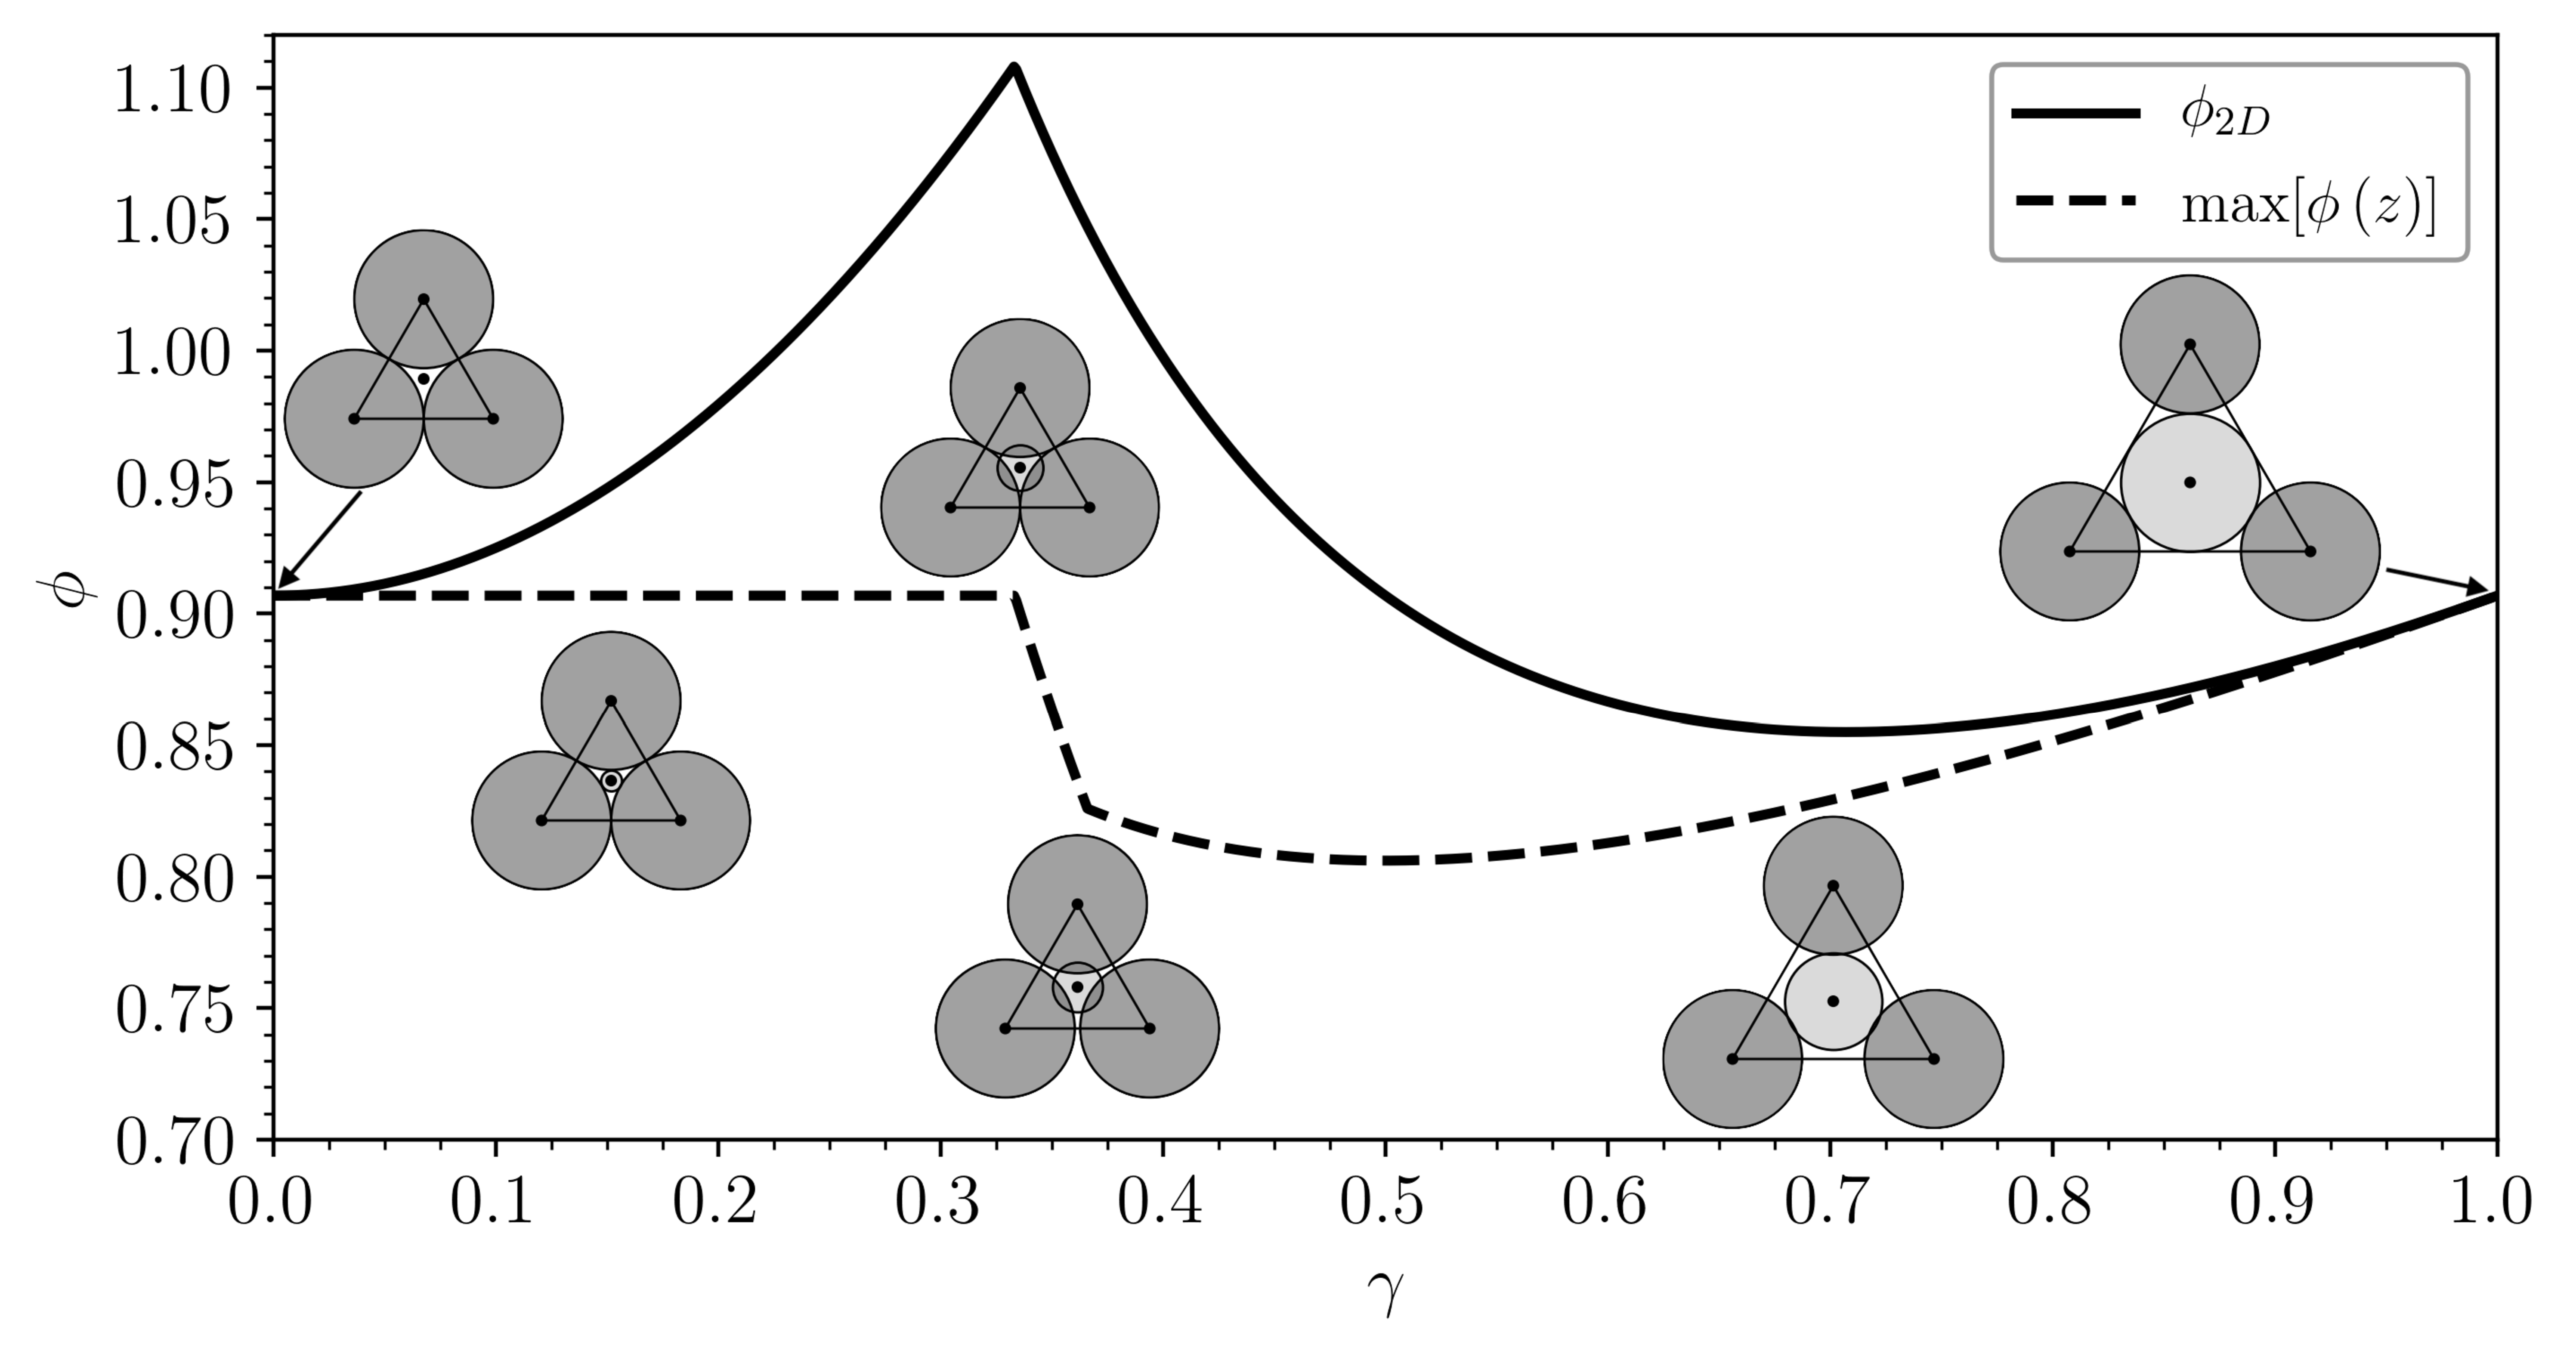
\includegraphics[width=0.75\textwidth]{./figures/quasi2d/max_packing.pdf}
	\caption{Variation in packing fraction for a binary crystal with varying radius ratio, $\gamma$. The packing fraction using the 2D definition is contrasted against that using the maximum packing with cut height.}
	\label{fig:crystalpackingfrac}
\end{figure}

For a polydisperse system, the explicit form of the second moment for the lognormal distribution can be calculated as,
\begin{align}
	\label{eq:wiid}
	\ewDii &= \frac{1}{\nDz}\int_{z/2}^\infty  \left(2Rz-z^2\right) f\left(R\right) \dd R \nonumber \\
	&= 2\langle \rs\rangle z\frac{N_D\left(ze^{-\sigma^2}\right)}{\nDz}-z^2\,.
\end{align}
There is a pleasing similarity between this result and equation \eqref{eq:radii}, and there there will be parity when $\sigma=0$ \ie{} the monodisperse limit. 
Intuitively, the form of the packing fraction with $z$ and its maximal value is independent of the number density and is instead solely a property of the sphere radii distribution. 

\section{Polydisperse Spheres}

The previous section explored theoretically properties of Voronoi diagrams in \qtd{} hard sphere systems.
The conclusions of that section are now tested numerically with monolayers of polydisperse spheres.
As with the mono\-- and bidisperse cases, the network properties are also analysed.
Systems at five different number densities in the range $\rho=0.00\rightarrow0.20$, are initialised with radii drawn from the lognormal distribution in equation \eqref{eq:lognormal}, with $\mu=0.0,\sigma=0.3$.
Configurations are then generated using the \mc{} technique outlined in section \ref{s:nonaddmc}.
Tessellations for each sample configuration can be made on-the-fly using both a weighted 2D Voronoi and the full 3D weighted Voronoi cut at a given height.
The periodicity in the system ensures that the Voronoi diagrams generated have no boundary, removing any potential edge effects. 
This maintains the mean polygon size of $\ki=6$, and ensures all node degrees are satisfied in the calculation of the assortativity.

It is important to note that because there are differing number of particles in the tessellations at a given cut height, care must be taken to ensure comparable statistical sampling for each state point. 
As discussed previously, the greater the cut height, the fewer particles there are with associated cells in the tessellation.
Therefore to ensure an equal number of cells are averaged for each value of $z$, simulations must be repeated with a different number of random seeds, proportional to  $1/\zN$.
This sampling also has an impact on the optimal number of particles to include.
If this number is too low the statistics will be affected at high $z$, regardless of number of starting seeds (\eg{} in the case where only a handful of particles are included in a 2D Voronoi, it becomes impossible to achieve a polygon with a large number of sides).
One must therefore balance these statistical considerations with the limits of computational efficiency.
In this section simulations included $\mathcal{N}=1000\rightarrow 5000$ particles, depending on cut height, so that all tessellations contained at least 50 cells, with a total of $\sim 10^7$ cells sampled for each state point.

To reiterate, the following different Voronoi methods will be compared:
\begin{enumerate}
	\item The section of a 3D Voronoi weighted with sphere radii, $\rs_i$, cut at height $z$.
	\item The sphere\--weighted 2D Voronoi weighted according to equation \eqref{eq:mapweights}.
	\item The disk\--weighted 2D Voronoi weighted according to equation \eqref{eq:radii}.
\end{enumerate}
As explained in section \ref{sec:vorrel} methods 1 and 2 are equivalent and produce identical results.
Method 3 on the other hand is expected to approximate to the other methods in the region near $z=0$.

\subsection{Cell Frequency and Packing Fraction}
\label{s:polycell}

To begin with, the number of cells that can be found in each tessellation is evaluated, as the cut height is increased; displayed in figure \ref{fig:nphia}\--\ref{fig:nphic}.
This is measured by the quantity $\zN$, the proportion of the total particles that have associated cells in the Voronoi construction.
For the sphere\--weighted Voronoi, figure \ref{fig:nphia}, the number of cells at a given cut height scales with the system density, such that a plot of $\nSz$ against $z\times \rho_0$ produces a near universal curve.
This curve is fit well by equation \eqref{eq:nsz} when $m=3$ \ie{} averaging over three nearest neighbours.
The curves for $m=2,4$ are also presented, lying either side of the $m=3$ curve, systematically under\-- and over\--estimating $\nSz$.
The main small discrepancy between systems of different density comes at the low cut heights, where the effects of short range ordering are still observable, as in \ref{fig:nphib}.
After the large initial drop in the number of cells at small cut heights, we see a long tail in the function $\nSz$.
This is indicative of the fact that the cells for the largest particles are very persistent.
As these particles are in low density and likely spaced far apart, the dividing planes are near\--vertical, leading to a slow convergence of the cell walls.

\begin{figure}

	\begin{subfigure}[b]{0.48\textwidth}
         \centering
         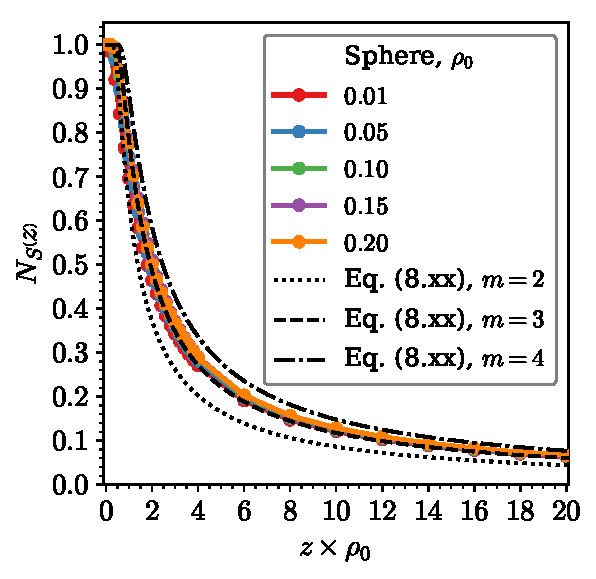
\includegraphics[width=\textwidth]{./figures/quasi2d/n_z_3d_sphere1.pdf}
         \caption{}
         \label{fig:nphia}
     \end{subfigure}
     \hfill
      \begin{subfigure}[b]{0.48\textwidth}
         \centering
         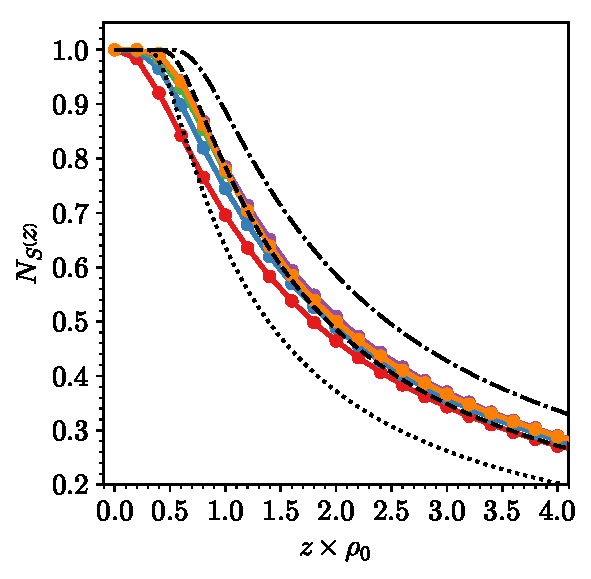
\includegraphics[width=\textwidth]{./figures/quasi2d/n_z_3d_sphere2.pdf}
         \caption{}
         \label{fig:nphib}
     \end{subfigure}
     \hfill
     
     \begin{subfigure}[b]{0.48\textwidth}
         \centering
         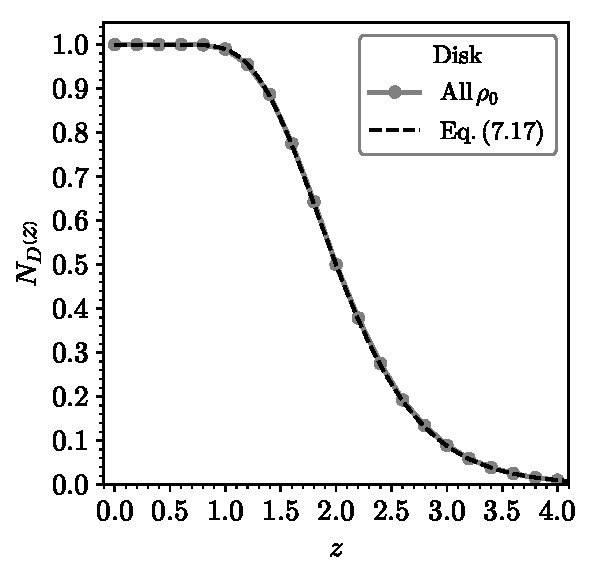
\includegraphics[width=\textwidth]{./figures/quasi2d/n_z_3d_disk.pdf}
         \caption{}
         \label{fig:nphic}
     \end{subfigure}
     \hfill
      \begin{subfigure}[b]{0.48\textwidth}
         \centering
         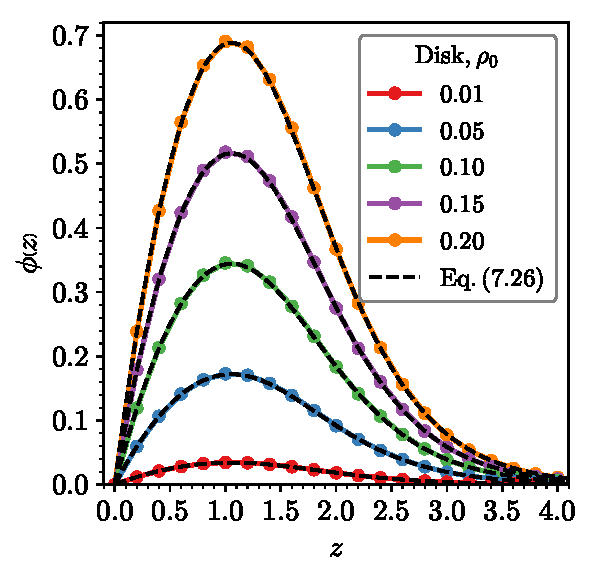
\includegraphics[width=\textwidth]{./figures/quasi2d/phi_z_2d.pdf}
         \caption{}
         \label{fig:nphid}
     \end{subfigure}
     \hfill
     
	\caption{Cell frequencies and packing fraction for Voronoi variants. Panels (a) and (c) compare the proportion of particles with cells in the sphere\-- and disk\-- weighted Voronoi tessellations respectively.
	Panel (b) gives a closer inspection of the data in panel (a) over the low $z$ range, using the same legend.
	Panel (d) gives the change in packing fraction as a function of the horizontal cut height.}
	\label{fig:nphi}
\end{figure}
\davidnote{Todo: update figure when equation numbers finalised}

For the disk\--weighted Voronoi, the behaviour in $\nDz$ is exactly described by equation \eqref{eq:ndz}.
In this case, the functional form is dependent only on the underlying particle distribution, and not the system density. 
In contrast to the sphere\--weighted case, the number of cells featured in these tessellations decays rapidly to zero beyond $\langle R\rangle$, simply reflecting that the maximum cell height is defined by the particle diameter, and so the polyhedra are truncated instead of extending above the particle.
Figure \ref{fig:nphid} explores the change in packing fraction as a function of the cut height, as explained in section \ref{s:qtdpackingfrac}.
As can be seen the fundamental shape is invariant to the number density, with $\rho_0$ merely acting as a scaling factor. 
Once again there is excellent agreement between the numerics and the theoretical results in equations \eqref{eq:altpackingfrac}.
Table \ref{tab:packingfrac} shows how the maximum packing fraction differs from the naive 2D packing fraction that can be calculated from the sphere radii and the cell area as in equation \eqref{eq:simplepackingfrac}.
Calculating packing fraction in this way always acts to reduce the overall number, and prevents the packing ever exceeding unity.

\begin{table}[h]
\caption{Difference between the maximum packing fraction as a function of height above the surface, and the 2D packing fraction using sphere radii for different number densities.}
\label{tab:packingfrac}
\centering
\begin{tabular}{ccc}
	\toprule
        $\rho$ & $\text{max}\left[\phi\left(z\right)\right]$ & $\phi_{2D}$ \\
        \midrule
	0.05 & 0.172 & 0.188 \\
	0.10 & 0.344 & 0.376 \\
	0.15 & 0.515 & 0.564 \\
	0.20 & 0.687 & 0.752 \\
	\bottomrule
\end{tabular}
\end{table}

\subsection{Network Properties}

The effects of the different methods of dividing space on the network properties of the system are also a subject of interest.
Previous studies which have compared the tessellations formed from cuts through 3D packings of mono- and bidisperse spheres have found differences when comparing the results of the different methods \cite{Oger2000,Gervois2004}.
For the different Voronoi methods discussed in this work, it is found that there is good agreement at low cut heights, but fundamental differences in the asymptotic limit as the cut height is increased.
The two network metrics common in this thesis are again compared for each system: the proportion of hexagons, $p_6$, and the assortativity, $\ass$, displayed in figure \ref{fig:pr}.
As expected there is good agreement between methods in both metrics at low cut height, with convergence in the limit of $z\rightarrow 0$.
However, at larger $z$ key differences emerge. 
The disk\--weighted Voronoi approaches the 2D Poisson\--Voronoi (PV) limit, $p_6\approx0.295$ and $r\approx -0.15$.
This is the limit which is obtained from having unweighted points randomly located in 2D space.
In contrast the sphere\--weighted Voronoi approaches a different, less well understood, limit with more diverse ring distribution and reduced ring\--ring correlations. We
will discuss the nature of this limit in a following section.

\begin{figure}

	\begin{subfigure}[b]{0.46\textwidth}
         \centering
         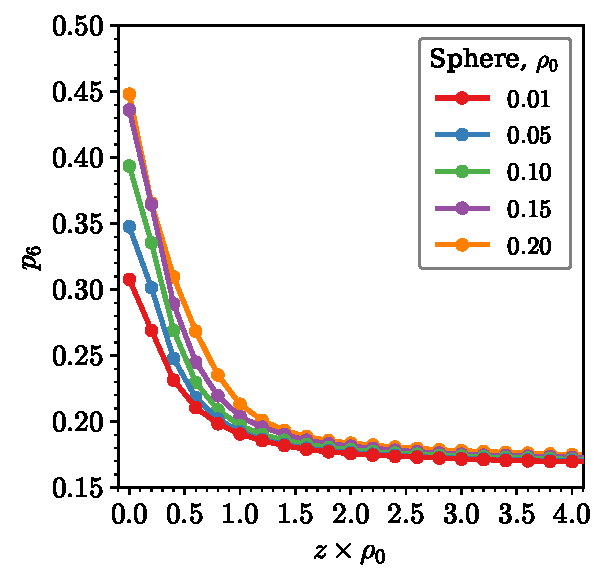
\includegraphics[width=\textwidth]{./figures/quasi2d/p6_z_3d_sphere.pdf}
         \caption{}
         \label{fig:pra}
     \end{subfigure}
     \hfill
     \begin{subfigure}[b]{0.48\textwidth}
         \centering
         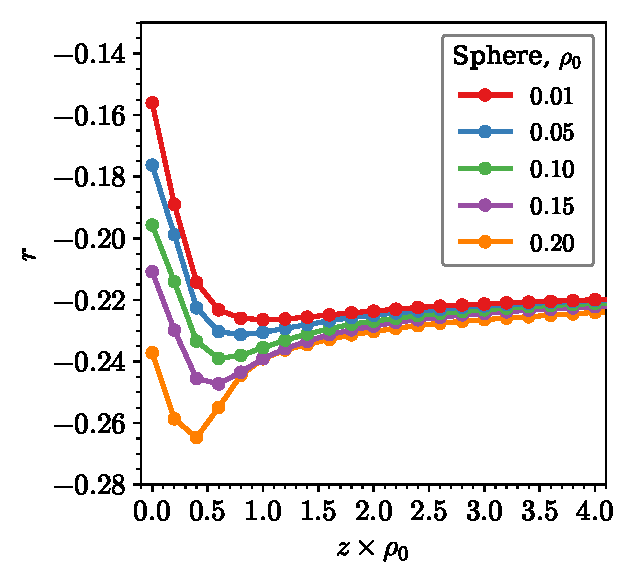
\includegraphics[width=\textwidth]{./figures/quasi2d/r_z_3d_sphere.pdf}
         \caption{}
         \label{fig:prb}
     \end{subfigure}
     \hfill
     
       \begin{subfigure}[b]{0.46\textwidth}
         \centering
         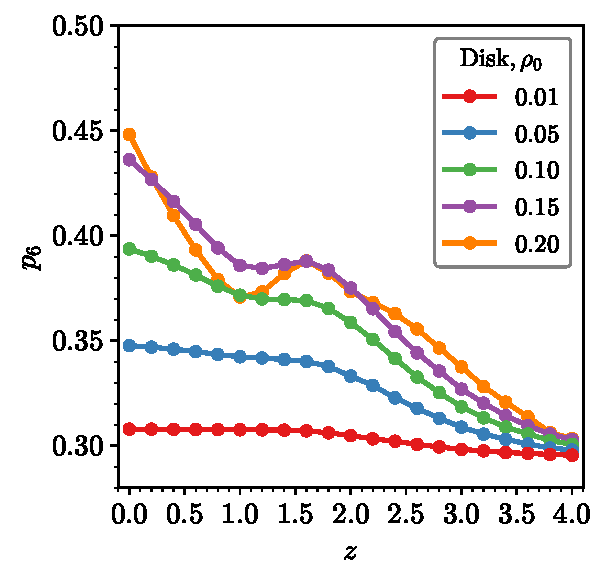
\includegraphics[width=\textwidth]{./figures/quasi2d/p6_z_3d_disk.pdf}
         \caption{}
         \label{fig:prc}
     \end{subfigure}
     \hfill
      \begin{subfigure}[b]{0.48\textwidth}
         \centering
         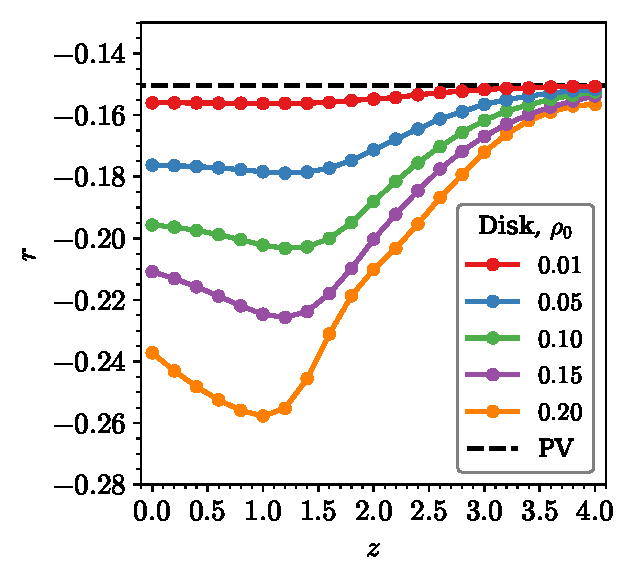
\includegraphics[width=\textwidth]{./figures/quasi2d/r_z_3d_disk.pdf}
         \caption{}
         \label{fig:prd}
     \end{subfigure}
     \hfill
     
	\caption{Comparison of the network properties in the sphere\--weighted and disk\--weighted Voronoi diagrams.
	The proportion of hexagons, $p_6$, and assortativity, $r$, with cut height is given in panels (a),(b) and (c),(d) for the sphere\-- and disk\--weighted diagrams respectively.}
	\label{fig:pr}
\end{figure}


To explain these observations two further measures are examined, the expected weight at a given cut height, $\langle w \rangle_z$, and the average nearest neighbour distance at a given cut height, $\ed$, given in figure \ref{fig:wd}.
These can be referred to in reference to equation \eqref{eq:radical}, which defines the position of the radical plane between two particles.
For the disk\--weighted Voronoi, it was showed above that the system approached the random PV limit.
In this limit the particles are randomly positioned and effectively unweighted. 
The only way this is achievable is if the inter\--particle distances scale in excess of the weightings with increasing cut height.
As seen from figures \ref{fig:wdc},\ref{fig:wdd}, this is indeed the case, with the distances increasing exponentially as the cut height exceeds an increasing number of particle diameters whilst the average weighting remains relatively constant.
Two further observations arise from these plots: equation \eqref{eq:ndist} describes the average distances very well (with the greatest deviation for higher density systems reflecting the presence of short range liquid structure), and the form of $\langle w_D\rangle_z$ mirrors the oscillations in the network properties.
These oscillations, which are particularly pronounced in $p_6$ (figure \ref{fig:prc}), are a result of the balance of weightings with cut height which become increasingly visible at higher densities where the inter\--particle distances are smaller.

Applying the same reasoning to the sphere\--weighted Voronoi, it is initially difficult to see how the network properties can tend to a limit which is \textit{not} PV.
However, this type of behaviour is not unknown, being similar to the observation that taking random sections through 3D PV polyhedra leads to 2D polygons which follow a distribution other than PV \cite{Hahn1994}.
As stated previously, as the cut height is increased particle cells are removed at random from the tessellation, so the system must be approaching some random limit.
Examining equation \eqref{eq:radical} again, the only way this cannot be PV is if the particle weightings scale in the same way as the inter\--particle distances.
Figure \ref{fig:wda} and \ref{fig:wdb} show that this is indeed the case, with both metrics scaling as $z^{1/2}$.
As such, the decreasing density of points is directly offset by the increase in weighting and a random limit other than PV is reached.

\begin{figure}

	\begin{subfigure}[b]{0.48\textwidth}
         \centering
         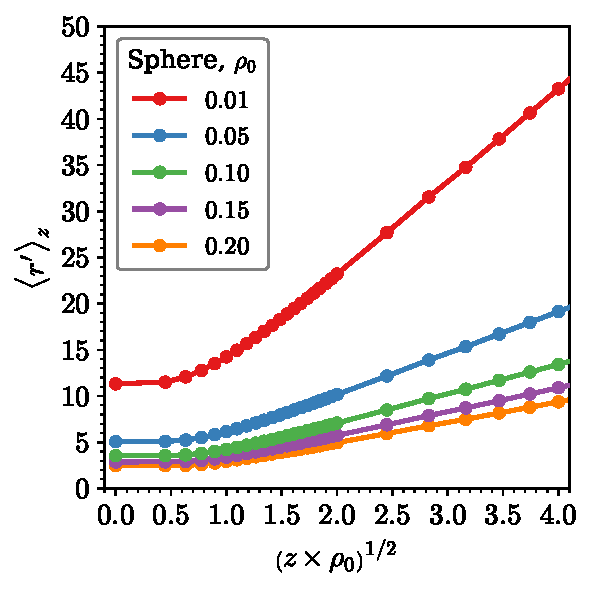
\includegraphics[width=\textwidth]{./figures/quasi2d/d_z_3d_sphere.pdf}
         \caption{}
         \label{fig:wda}
     \end{subfigure}
     \hfill
	\begin{subfigure}[b]{0.48\textwidth}
         \centering
         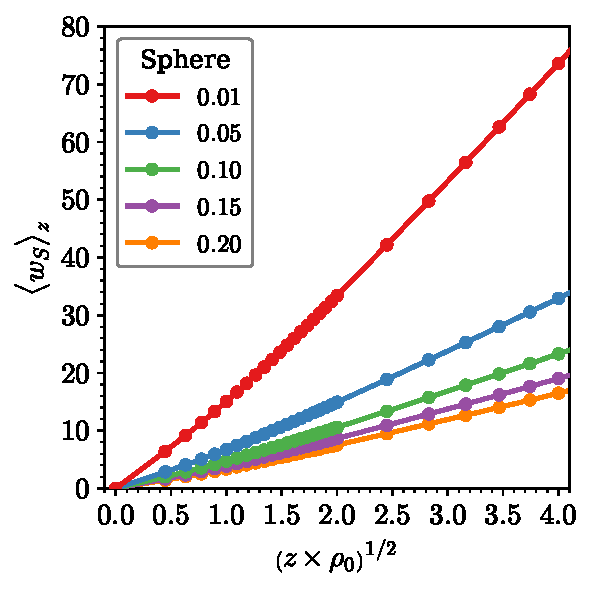
\includegraphics[width=\textwidth]{./figures/quasi2d/w_z_3d_sphere.pdf}
         \caption{}
         \label{fig:wdb}
     \end{subfigure}
     \hfill     
     
     \begin{subfigure}[b]{0.48\textwidth}
         \centering
         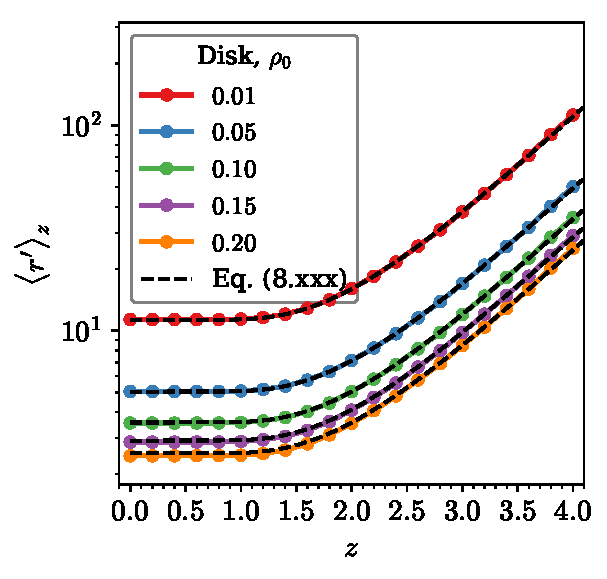
\includegraphics[width=\textwidth]{./figures/quasi2d/d_z_3d_disk.pdf}
         \caption{}
         \label{fig:wdc}
     \end{subfigure}
     \hfill
      \begin{subfigure}[b]{0.48\textwidth}
         \centering
         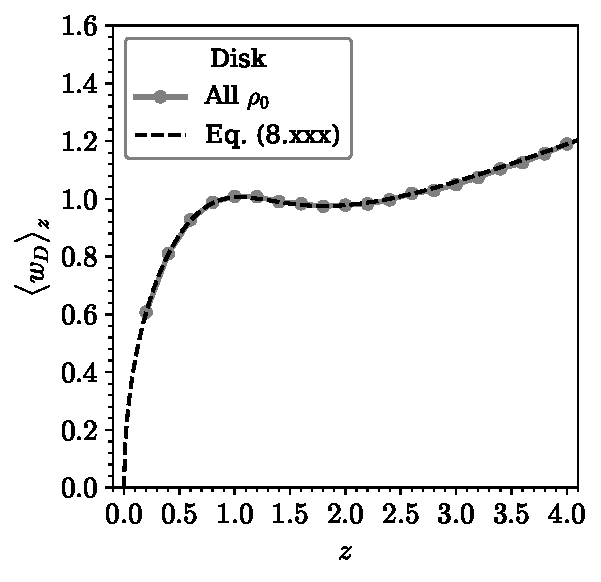
\includegraphics[width=\textwidth]{./figures/quasi2d/w_z_3d_disk.pdf}
         \caption{}
         \label{fig:wdd}
     \end{subfigure}
     \hfill
	
	\caption{Comparison of the inter\--particle distances (panels(a),(c)) and particle weights (panels (b),(d)) for the sphere\-- and disk\--weighted Voronoi at increasing cut heights. In the sphere\--weighted case both measures scale as $z^{1/2}$ in the high cut height limit, whereas in the disk\--weighted case the inter\--particle distance increases exponentially, making the weighting effect negligible.}
	\label{fig:wd}
\end{figure}

\section{Experimental Interpretation}

Having examined the numerical results for qtd{} hard sphere monolayers, the practical conclusions for experimentation can be briefly summarised.
As mentioned previously, for those studying quasi\--2D systems experimentally, it is often preferable to analyse configurations using particle positions projected into the $x\--y$ plane, using a 2D Voronoi method.
Not only is this more practicable, it is also leads to straightforward visualisation and analysis.
The most common approach is therefore to use a unweighted 2D Voronoi.
This is understandable, as it requires no knowledge of the particle radii, which maybe prove difficult to accurately determine.
With bi\-- or polydisperse particle systems, it was previously unclear that the unweighted 2D Voronoi analysis was in fact wholly appropriate, given that for true 2D systems (\eg{} polydisperse disks) it is known to allocate space disproportionately. 
 
However, in the second half of this chapter it has been shown that possibly contrary to expectation, the use of an unweighted 2D Voronoi analysis, for polydisperse particles sedimented on a plane, is completely valid and well defined.
The unweighted 2D Voronoi is topologically equivalent to the tessellation formed by taking the basal faces of the polyhedra formed from the fully \textit{weighted} 3D Voronoi diagram.
Therefore, in the absence of the information about particle radii, the unweighted 2D Voronoi can still be mapped to the basal section through the weighted 3D diagram.
In addition, for such quasi\--2D systems, the unweighted 2D Voronoi diagram may be considered the best construction possible. 
This is because it corresponds to the only section through the 3D weighted Voronoi which is guaranteed to include a cell for each particle; notwithstanding the fact that it is also the simplest Voronoi method to implement and evaluate.
As an aside, this section also seems to maximise the proportion of hexagons rings in the tessellation.

Furthermore, the more general stereology problem has been considered for quasi\--2D systems, which is a subject of interest in similar studies of polycrystalline materials  \cite{Falco2017,Depriester2019}.
Here it has been demonstrated that the horizontal 2D sections through the 3D weighted Voronoi diagram can be calculated using a 2D weighted Voronoi, with weightings given in equation \eqref{eq:mapweights}.
Therefore, if the particle radii are known, one can easily calculate the 2D sections at a given cut height.
This is convenient as such computational methods are more readily available than cutting the 3D weighted Voronoi directly, which is a non\--standard technique.

Finally an alternative definition of the packing fraction has been introduced by considering the quasi\--2D system as a series of hard disk tessellations.
This packing fraction is well defined in that it cannot exceed unity and does not require an arbitrary definition of the sample volume.

\section{Chapter Conclusions}

The role of the Voronoi construction in the analysis of \qtd{} hard sphere systems has been extensively explored.
A substantial part of this work has been a theoretical study of the relationships between various 2D and 3D tessellations for \qtd{} systems.
Although some of the problems investigated are more fundamental, others are of direct relevance to ongoing experimental research.
Most significantly, a link has been drawn between the application of an unweighted 2D Voronoi construction and a 3D construction in which the division of space is weighted in terms of particle size, for the case in which the spheres sit on a surface.
As a result, a clear geometrical meaning has been provided to the commonly used unweighted 2D Voronoi diagram; showing it to be equivalent to the tessellation 
formed from taking the basal polygons in the 3D Voronoi diagram weighted by the sphere 
radii.

As an application of this, experimental configurations of \qtd{} colloidal monolayers of varying parameters were analysed using Voronoi techniques.
The results of these analyses were also compared to analogous configurations generated by non\--additive hard disk \mc{}, to which there was good agreement.
Monodisperse systems were found to have ring statistics concordant with \lm's law and network assortativity which was linear in packing fraction.
Bidisperse systems were considered in terms of the partial properties of the two sphere components.
The partial ring size distributions were shown to be fit well by maximum entropy distributions and can be tuned through varying the system parameters of packing fraction, composition and radius ratio.


